% PLANTILLA Y GUÍA DEL TRABAJO ESCRITO
% ------------------------------------

\immediate\write18{makeindex -s nomencl.ist -o "proyecto.nls" "proyecto.nlo"}

% Tipo de documento
\documentclass[final]{proyectoelectronico}

% A. PAQUETES Y MACROS ESPECIALES -------
% Paquetes y definiciones que no están incluidos 
% en la clase proyectoelectrico.cls o que son 
% propios del proyecto.
% -----------------------------------------
% OTROS PAQUETES E INSTRUCCIONES ESPECIALES
% -----------------------------------------

% PAQUETES
%%%%%%%%%%

% Para insertar PDFs
\usepackage{pdfpages}
% Para insertar código fuente estilizado
\usepackage{listings}
	\lstset{basicstyle=\ttfamily,
    		breaklines=true,
            numbers=left, 
    		numberstyle=\tiny, 
    		stepnumber=1, 
    		numbersep=6pt
            }

% Para adjuntar pdf
\usepackage{pdfpages}

% Para usar múltiples columnas
\usepackage{multicol}

% Para crear árboles conceptuales
\usepackage{forest}

% Para insertar símbolos extraños
\usepackage{marvosym}

% Para insertar texto fútil
\usepackage{lipsum}

% NUEVAS INSTRUCCIONES
%%%%%%%%%%%%%%%%%%%%%%

\newcommand{\EIEx}{\textsc{Escuela \Lightning~ Ingeniería Eléctrica}}

% Definición de algunos símbolos matemáticos
\newcommand{\me}{\mathrm{e}}
\newcommand{\mi}{\mathrm{i}}
\newcommand{\mj}{\mathrm{j}}
\newcommand{\md}{\mathrm{d}}

% Listas con menos espacio entre ítemes (más ajustado)
\newcommand{\ajustado}{\itemsep0pt\parskip0pt\parsep0pt}

% FORMATO PARA EL REGLAMENTO
%%%%%%%%%%%%%%%%%%%%%%%%%%%%

\newcounter{articulo}
\newcommand{\articulo}[2]{
	{
    \stepcounter{articulo}
    \noindent
	\textbf{Artículo \thearticulo} --- \textit{#1}
	\vspace{2mm}\\
	}{
	#2
	\vspace{2mm} \\
	}
}

\newcounter{capitulo}
\newcommand{\capitulo}[1]{
	{
    \stepcounter{capitulo}
    \centering\large\bfseries
    Capítulo \Roman{capitulo}. #1
    \vspace{4mm}\\
    }
}

\hypersetup{
    pdfauthor={MODIFICAR Grupo X 2023},
    pdftitle={Digitalización de Control Analógico para Fuente de Alimentación Ajustable},
    pdfsubject={Informe Final PyDE},
    pdfkeywords={PyDE, Fuente de Alimentación, Control Digital},
    pdfproducer={LaTeX},
    pdfcreator={pdflatex}
}

% Tipografía
\usepackage{libertine}
\usepackage{libertinust1math}
\usepackage[T1]{fontenc}
\renewcommand*{\ttdefault}{cmtt}
\newcommand{\entreComillas}[1]{“#1”} % para que esté entre comillas
\newcommand{\listaVacio}{Varios} % celda vacia de la lista de componentes 

%---------------------------------------

% B. DATOS ------------------------------
% Todos los nombres incluyen dos apellidos,
% acentos y signos de puntuación apropiados.
% Revisar las recomendaciones sobre el título
% y los nombres de los profesores en la guía.

% Título del proyecto
\titulo{Digitalización de Control Analógico para Fuente de Alimentación Ajustable}

% Autor (nombre y carné)
\autoruno{Korpys Ernesto Andrés}
\carneuno{K-3290/5} % legajo
\emailuno{ernesto.korpys@gmail.com}

\autordos{Fernando Natanael Krindgester}
\carnedos{MODIFICAR Legajo del autor 2} % legajo
\emaildos{krindgesfer@gmail.com}

%\autortres{Nombre del tercer integrante}
%\carnetres{Legajo del tercer integrante} % legajo
%\emailtres{Email del tercer integrante}

% Tutores (nombre y correo)

\tutoruno{Botterón Fernando}
\tutemailuno{botteron@fio.unam.edu.ar}

\tutordos{Maxit Alejandro Germán}
\tutemaildos{alejandro.maxit@fio.unam.edu.ar}

% Profesor(a) guía
\guia{Ricardo Andrés Korpys}

% Profesores lectores 
\lectorA{Guillermo Alfredo Fernandez}
\lectorB{Alejandro Germán Maxit}

% Fecha de entrega del trabajo escrito
\mes{11}	% Número del mes
\ano{2024}	% Formato AAAA
% ---------------------------------------

% C. CONTENIDOS -------------------------

%\hypersetup{citecolor=black} % esto es el color en el que aparecen las citas cuando se usa el comando \cite{}, por defecto las llaves están el negro y el número en azul

%%%%%%%%%%%%%%%%%%%
\begin{document}
%%%%%%%%%%%%%%%%%%%

\frontmatter

% 1. PORTADA
\portada

% 2. HOJA DE APROBACIÓN
\iffinal
\aprobacion
\fi

% 3. RESUMEN (EN ESPAÑOL E INGLÉS)
% EL RESUMEN
% ----------

\begin{resumen}{Fuente de tensión, Lazo de control, DSP, digital,}

El proyecto se centra en la modernización de una fuente de alimentación preexistente, en su mayoría analógica, de una tensión variable desde 0V hasta 30V y una corriente ajustable desde 0A hasta 3A, mediante la implementación de un control digital para la regulación precisa de la tensión y corriente de salida, así como la implementación de lazos de control digital para garantizar la estabilidad de la salida en diversas condiciones de carga. 
La esencia de este proyecto radica en la utilización de un controlador digital de señales para ajustar la salida de la fuente de alimentación, a través de un teclado. Este enfoque proporciona al usuario la capacidad de configurar fácilmente los valores deseados de tensión y corriente de salida, mientras que un display integrado ofrece una retroalimentación visual en tiempo real, mostrando tanto los valores establecidos como los valores reales de salida.
Como núcleo de control, se emplea el controlador digital de señales dsPIC30F4011 (40-Pin PDIP), destacando su capacidad para gestionar eficientemente las operaciones del sistema. Es importante mencionar que este diseño no requiere de conexión inalámbrica, lo que simplifica su implementación y uso.


\end{resumen}

% EL RESUMEN EN INGLÉS
% --------------------

\begin{theabstract} {Direct Current Power Supply:\\Digitization of Analog Control for adjustable Power Supply} {Voltage source, Control loop, DSP, Digital}

The project focuses on modernizing an existing power supply, predominantly analog, with a variable voltage range from 0V to 30V and an adjustable current range from 0A to 3A. This is achieved through the implementation of digital control for precise regulation of both voltage and current output, alongside the incorporation of digital control loops to ensure output stability under various load conditions.

The essence of this project lies in the utilization of a digital signal controller to adjust the power supply's output via a keypad. This approach grants users the ability to easily configure desired voltage and current values, while an integrated display provides real-time visual feedback, showcasing both set and actual output values.

At the core of control, the project employs the Arduino NANO, notable for its efficient management of system operations. It is pertinent to mention that this design does not necessitate wireless connectivity, simplifying its implementation and usage.

\section*{Objectives}

\begin{itemize}
    \item Power supply providing a variable output voltage from 0V to 30V and an adjustable current from 0A to 3A.
    \item Implement digital control loops to ensure the regulation of output voltage and current, maintaining stability under various load conditions.
    \item Allow easy and precise configuration of output voltage and current using an input system, such as a rotary encoder or a keypad.
    \item Integrate a display showing both user-set values and actual output values, providing real-time visual feedback.
    \item Ensure complete galvanic isolation between the power stage and digital control, ensuring system safety and reliability.
    \item Wireless connectivity is not required.
\end{itemize}

\end{theabstract}

% El entorno 'theabstract' tiene el formato \begin{theabstract}{A} ...B... \end{theabstract} donde A es el título del proyecto traducido de inglés a español y B es el contenido, en inglés, del resumen. Se recomienda buscar ayuda calificada para la elaboración y/o revisión de este resumen.

% 4. RECONOCIMIENTOS
\iffinal
% LOS RECONOCIMIENTOS
% -------------------

% Aquí se escribe la dedicatoria del proyecto y los agradecimientos. El entorno 'reconocimiento' tiene la estructura \begin{reconocimiento}{Dedicatoria} Agradecimientos \end{reconocimiento}

\begin{reconocimiento}{Dedicado a nuestras familias y amigos Saludos.}

Korpys Ernesto.
Agradezco de corazón a mi familia por su inquebrantable apoyo a lo largo de toda mi vida. En especial, a mi madre Gladys, cuyo amor y sacrificio han sido mi mayor inspiración y motor para alcanzar mis metas.
Agradezco enormemente a mi compañero de proyecto, Fernando, quien no solo fue mi compañero de trabajo, sino también un amigo invaluable durante esta travesía académica. Su colaboración y compañerismo fueron fundamentales para el éxito de este proyecto.
A mis amigos presentes, les doy las gracias por su constante ánimo y respaldo, por compartir conmigo momentos de alegría y por ser un pilar fundamental en mi vida.
Expreso mi profundo agradecimiento al equipo docente, a los ingenieros Botteron, Fernandez y Kolodziej, quienes no solo compartieron su conocimiento y experiencia conmigo, sino que también me brindaron su apoyo académico cuando más lo necesité. Gracias por ser guías en este viaje de aprendizaje y crecimiento profesional.


\end{reconocimiento}
\fi

% 5. TABLAS DE CONTENIDO, FIGURAS Y TABLAS
\tableofcontents
\listoffigures
\listoffotos
\listoftables
%\lstlistoflistings

% 6. NOMENCLATURA
%\input{nomenclature.tex}
\nomenclature{$R$}{Resistencia eléctrica}
% LA NOMENCLATURA
% ---------------

% La nomenclatura se realiza con el paquete 'nomencl'. Para ingresar un nuevo elemento, se debe usar el comando \nomenclature{símbolo}{definición}, ya sea en este archivo nomenclatura.tex (más fácil para encontrar y editar), o en cualquier parte del documento (probablemente cuando se introduce una nueva variable o constante). Para más opciones del paquete, favor referirse a su documentación (https://www.ctan.org/pkg/nomencl). También hay una buena guía de uso en https://www.sharelatex.com/learn/Nomenclatures.

% Formato recomendado
% -------------------

% Variable o constante matemática
% \nomenclature{$V$}{Tensión eléctrica}

% Acrónimo
% \nomenclature{TBH}{Para ser honesto (del inglés \textit{To Be Honest})}

% Si únicamente existen acrónimos del inglés, se puede omitir la frase 'del inglés'. La definición no tiene punto al final.

\nomenclature{$R$}{Resistencia eléctrica}
\nomenclature{$I$}{Corriente eléctrica}
\nomenclature{$V$}{Tensión eléctrica}
\nomenclature{IEEE}{Instituto de Ingenieros Eléctricos y Electrónicos (del inglés \textit{Institute of Electrical and Electronics Engineers})}
\nomenclature{FIO}{Facultad de Ingeniería}
\nomenclature{UNaM}{Universidad Nacional de Misiones}
\nomenclature{ROM}{Read Only Memory}
\nomenclature{RAM}{Random Access Memory}
\nomenclature{CMOS}{Complementary Metal-Oxide Semiconductor}
\nomenclature{E/S}{Entrada/Salida}
\nomenclature{TTL}{Transistor-Transistor Logic}
\nomenclature{I\textsuperscript{2}C}{Inter-Integrated Circuit}
\nomenclature{UART}{Universal Asynchronous Receiver-Transmitter}
\nomenclature{SPI}{Serial Peripheral Interface}
\nomenclature{COSMAC}{Complementary Symmetry Monolithic Array Computer}
\nomenclature{MSB}{Most Significant Bit}
\nomenclature{LSB}{Least Sifnificant Bit}
\nomenclature{EPROM}{Erasable Programmable Read-Only Memory}
\nomenclature{EEPROM}{Electrically Erasable Programmable Read-Only Memory}
\nomenclature{RCA}{Radio Corporation of America}
\nomenclature{EDA}{Electronic Design Automation}
\nomenclature{$VEEEEE$}{asdasdasdas eléctrica}
\nomenclature{PCB}{Circuito impreso (del inglés \textit{Printed Circuit Board})}
\nomenclature{PAL}{Programmable Array Logic}
\nomenclature{GAL}{Generic Array Logic}
\nomenclature{PLC}{Programmable Logic Controller}
\nomenclature{KiCad}{Software para el diseño de esquemáticos y PCBs de circuitos electrónicos}
\nomenclature{MRD}{Memory Read}
\nomenclature{MWR}{Memory Read}

\printnomenclature
\mainmatter

% 7. CAPÍTULOS
% ----------------------
  \chapter{Introducción}
% ----------------------

\label{C:introduccion}

El proyecto se centra en la modernización de una fuente de alimentación preexistente, en su mayoría analógica, de una tensión variable desde 0V hasta 30V y una corriente ajustable desde 0A hasta 3A, mediante la implementación de un control digital para la regulación precisa de la tensión y corriente de salida, así como la implementación de lazos de control digital para garantizar la estabilidad de la salida en diversas condiciones de carga. \par
La esencia de este proyecto radica en la utilización de un controlador digital de señales para ajustar la salida de la fuente de alimentación, introduciendo el valor deseado a través de un teclado o un encoder rotativo. Este enfoque proporciona al usuario la capacidad de configurar fácilmente los valores deseados de tensión y corriente de salida, mientras que un display integrado ofrece una retroalimentación visual en tiempo real, mostrando tanto los valores establecidos como los valores reales de salida.\par
Como núcleo de control, se emplea el microcontrolador digital Arduino NANO, destacando su bajo costo, accesibilidad y la disponibilidad de librerías creadas por la gran comunidad que lo respalda. Resulta importante mencionar que este diseño no requiere de conexión inalámbrica, lo que simplifica su implementación y uso.
 \cite{plantilla_universidad_de_costa_rica}. \par 



%%%%%%%%%%%%%%%%%%%%%%%%%%%%%%%%%%%%%%%%%%%%%%


\chapter{Introducción teórica a fuentes DC}
% ----------------------

\label{C:Fuentes de corriente continua}

\section{Sobre las fuentes de alimentación.}
Las fuentes de alimentación electrónicas se definen como circuitos que transforman la potencia eléctrica de entrada, ya sea de corriente alterna (CA) o de corriente continua (CC), en potencia de salida, ya sea de corriente alterna (CA) o de corriente continua (CC). Esta definición excluye así a las fuentes de alimentación basadas en los principios de máquinas rotativas y distingue las fuentes de alimentación de la categoría más general de fuentes de energía eléctrica que derivan la potencia eléctrica de otras formas de energía (por ejemplo, baterías, celdas solares, celdas de combustible). Las fuentes de alimentación electrónicas se pueden dividir en cuatro amplias clasificaciones:

\begin{enumerate}
    \item CA de entrada, CA de salida regulada por línea o cambiadores de frecuencia.
    \item CC de entrada, CC de salida convertida o regulada.
    \item CC de entrada, CA de salida de corriente alterna, conocidas como inversores.
    \item CA de entrada, CC de salida.
\end{enumerate}

Esta última categoría es, con mucho, la más común de las cuatro y generalmente es a la que se hace referencia cuando se habla de una "fuente de alimentación". Las fuentes de alimentación de CC de salida pueden proporcionar cuatro salidas básicas o modos de operación:

\begin{itemize}
    \item Voltaje Constante: El voltaje de salida se mantiene constante a pesar de los cambios en la carga, la línea o la temperatura.
    \item Corriente Constante: La corriente de salida se mantiene constante a pesar de los cambios en la carga, la línea o la temperatura.
    \item Límite de Voltaje: Igual que el voltaje constante excepto por características de regulación menos precisas.
    \item Límite de Corriente: Similar a la corriente constante excepto por una regulación menos precisa.
\end{itemize}
Como se explica en esta sección, las fuentes de alimentación están diseñadas para ofrecer estas salidas en diversas combinaciones para diferentes aplicaciones. [3]
La analizada en este informe será una fuente CA entrada CC salida con control de voltaje y límite de corriente.

\subsection{Fuente ideal de  tensión.}
No existe tal cosa como un dispositivo perfecto en la electrónica, sin embargo con el fin de buscar la excelencia en el diseño y producción de un prototipo de fuente se parte del principio de que característica debería contar la misma para estar lo más próxima a este escenario hipotético. Todo esto lleva a decir que una fuente de alimentación de voltaje constante ideal sería aquella que tendría una impedancia de salida cero en todas las frecuencias. Por lo tanto, el voltaje permanece perfectamente constante a pesar de cualquier cambio en la corriente de salida demandada por la carga.
Una simple fuente de alimentación no regulada compuesta únicamente por un rectificador y un filtro no es capaz de proporcionar un voltaje de salida de corriente continua sin ondulaciones cuyo valor permanece razonablemente constante. Para obtener siquiera una aproximación básica de la característica de salida ideal, algún tipo de elemento de control (regulador) debe incluirse en la fuente. [3]

\begin{figure}
    \centering
    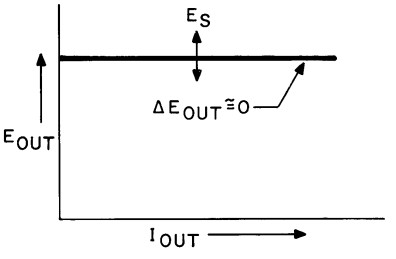
\includegraphics[scale=0.4]{./imagenes/salidaidealfuentedc.jpg}
    \caption{Voltaje de tensión constante salida de fuente ideal.}
    \label{F:estructura_archivos}
\end{figure}

\subsection{Técnicas de Regulación}
La mayoría de las fuentes de alimentación de voltaje constante actuales emplean una de estas cuatro técnicas de regulación:
\begin{itemize}
    \item Serie (Lineal).
    \item Pre-regulador/Regulador en Serie.
    \item Conmutación.
    \item SCR.
\end{itemize}
Sin embargo, el objetivo de este documento escapa a explicar a detalle entre cada uno de estos modelos por lo que este se limitará a mencionarlas y a mencionar el que supera a los demás en relevancia para este documento. 
\subsection{Fuentes de alimentación Lineales.}
Las fuentes de alimentación lineales son un elemento fundamental en la mayoría de los dispositivos electrónicos que utilizamos en nuestra vida cotidiana. Estas fuentes proporcionan la energía necesaria para alimentar circuitos electrónicos, convirtiendo la energía de la red eléctrica en una forma utilizable y estable para los componentes electrónicos. En esta sección, explicaremos los elementos clásicos básicos que componen las fuentes de alimentación lineales y su funcionamiento fundamental para más adelante entrar en profundidad sobre la fuente que concierne a este informe.

\section{Funcionamiento básico.}
El tipo más simple y común de fuentes de alimentación de corriente continua (CC) es un sistema "lineal", mostrado esquemáticamente en la fig . Primero, se utiliza un transformador para "reducir" la tensión de línea de CA a un voltaje pico más pequeño, que generalmente es aproximadamente 2-3 voltios más grande que el voltaje de salida de CC deseado. Un circuito de diodos rectifica la señal de CA, produciendo una forma de onda con una gran componente de CC. Luego, se utiliza un banco de filtros de condensadores para "suavizar" o "filtrar" la sinusoidal rectificada. Bajo condiciones de carga normales, siempre hay alguna variación periódica residual o "ripple" en la señal filtrada. Si la aplicación requiere un ripple muy bajo y una salida de CC constante sobre un amplio rango de condiciones de carga, entonces se requiere regulación activa para reducir o eliminar aún más este ripple residual. [2]
\begin{figure}
    \centering
    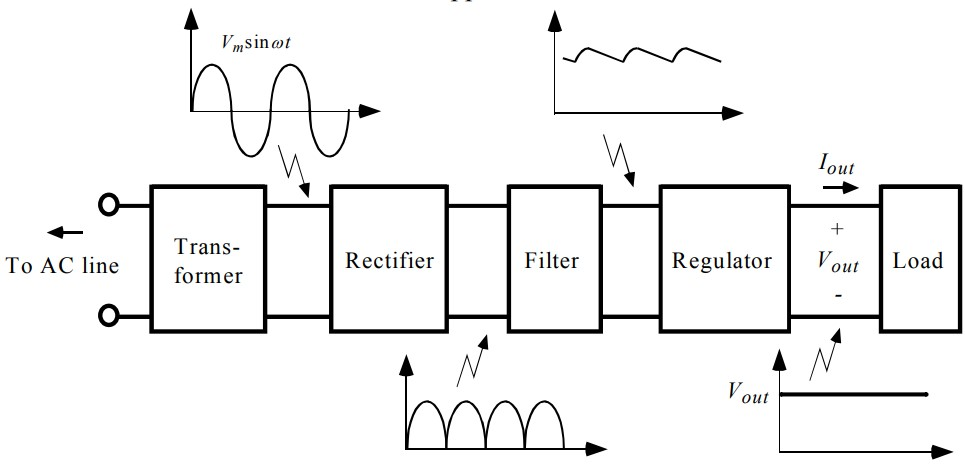
\includegraphics[scale=0.5]{./imagenes/componentesFL.jpg}
    \caption{Partes de una fuentes de tensión.}
    \label{F:estructura_archivos}
\end{figure}

\subsection{Transformador}
El transformador es uno de los componentes principales de una fuente de alimentación lineal. Su función principal es transformar la corriente alterna (CA) de la red eléctrica en una corriente alterna con un voltaje específico adecuado para la aplicación. Consiste en dos bobinas de alambre enrolladas alrededor de un núcleo de hierro, donde la relación entre el número de vueltas en las bobinas determina la relación de transformación del voltaje.

\subsection{Rectificador}
El rectificador es otro componente esencial que convierte la corriente alterna en corriente continua (CC). Esto se logra mediante diodos rectificadores, que permiten que la corriente fluya en una sola dirección. Los rectificadores pueden ser de media onda o de onda completa, dependiendo de cómo se utilizan los diodos para rectificar la señal de entrada.

\subsection{Filtro}
Después de que el rectificador convierte la corriente alterna en corriente continua, la señal resultante puede contener fluctuaciones no deseadas o rizado. Para eliminar estas fluctuaciones y obtener una salida de voltaje suave y constante, se utiliza un filtro. El filtro puede estar compuesto por capacitores y bobinas para eliminar el rizado y suavizar la salida de voltaje.

\subsection{Regulador}
El regulador es el componente final de una fuente de alimentación lineal y se utiliza para mantener constante la salida de voltaje independientemente de las variaciones en la entrada de voltaje o en la carga. Los reguladores de voltaje pueden ser de tipo lineal, que controlan la cantidad de energía disipada como calor para mantener el voltaje de salida constante, o de tipo conmutado, que regulan el voltaje de salida ajustando el ciclo de trabajo de un interruptor.

\section{Ventajas y desventajas}
Todo dispositivo cuenta con una serie de características que la hacen una opción dominante por sobre las demás. Aquí se listan los detalles más dominantes de las fuentes de tensión lineal que las podría hacer sugeribles frente a otro tipo de configuraciones.
Ventajas.
\begin{itemize}
    \item Simplicidad: Son relativamente simples en diseño y operación.
    \item Bajo ruido: Tienen un nivel de ruido más bajo en comparación con algunas otras formas de fuentes de alimentación.
    \item Baja interferencia electromagnética (EMI): Emiten menos interferencia electromagnética en comparación con las fuentes de alimentación conmutadas.
    \item Buen rendimiento en aplicaciones de baja potencia: Son eficientes y efectivas en aplicaciones de baja potencia.
    \item Buena regulación: Suelen tener una regulación de voltaje estable y precisa.
\end{itemize}
Desventajas.
\begin{itemize}
    \item Baja eficiencia energética: Tienen una eficiencia energética más baja en comparación con las fuentes de alimentación conmutadas, especialmente en aplicaciones de alta potencia.
    \item Disipación de calor: Tienden a generar más calor durante la operación debido a la regulación de voltaje a través de dispositivos de regulación lineal, lo que puede requerir disipadores de calor o ventilación adicional.
    \item Mayor tamaño y peso: Suelen ser más grandes y pesadas en comparación con las fuentes de alimentación conmutadas con la misma capacidad de potencia.
    \item Menor rango de voltaje de entrada: Tienen un rango de voltaje de entrada limitado en comparación con las fuentes de alimentación conmutadas, lo que puede limitar su aplicabilidad en ciertos entornos o condiciones de operación.
\end{itemize}

\section{Evolución y mejoras con el pasar de los años}
Las fuentes de corriente directa (DC) han experimentado una evolución significativa desde sus inicios, impulsadas por avances tecnológicos que han mejorado su eficiencia, fiabilidad y capacidad de adaptación a diversas aplicaciones. A lo largo de los años, estas mejoras han permitido que las fuentes de DC se conviertan en componentes esenciales en una amplia gama de dispositivos electrónicos y sistemas de energía. Las mejoras no solamente abarcan mejores materiales sino también el uso de estrategias de control más inteligentes y adaptación para entornos específicos.
Algunas de estas mejoras son:
\begin{itemize}
    \item \textbf{Tecnología de Conversión de Energía}: Las fuentes de DC modernas utilizan técnicas avanzadas de conversión de energía, como la conmutación de alta frecuencia, que permiten una mayor eficiencia energética y una reducción en el tamaño de los dispositivos. La tecnología de conversión resonante, como los convertidores LLC (Inductor-Inductor-Capacitor), ha mejorado la eficiencia en aplicaciones de alta potencia al minimizar las pérdidas por conmutación \cite{zhang2013}.
    \item \textbf{Materiales de Banda Ancha}: La incorporación de materiales semiconductores de banda ancha, como el carburo de silicio (SiC) y el nitruro de galio (GaN). Estos materiales permiten operar a mayores voltajes y frecuencias, mejorando la eficiencia y reduciendo las pérdidas térmicas. Los dispositivos basados en SiC y GaN son especialmente beneficiosos en aplicaciones de alta potencia y alta densidad \cite{palmour2019}.
    \item \textbf{Integración de Funcionalidades Inteligentes}: Las fuentes de DC actuales incorporan funcionalidades inteligentes, como el monitoreo y control digital en tiempo real, que optimizan el rendimiento y la eficiencia energética. Estas fuentes pueden ajustar dinámicamente sus parámetros de operación en respuesta a las condiciones de carga, mejorando así la fiabilidad y prolongando la vida útil de los componentes conectados \cite{brown2020}.
    \item \textbf{Reducción del Tamaño y Peso}: Los avances en diseño y materiales han permitido la reducción significativa del tamaño y peso de las fuentes de DC. Esto es crucial en aplicaciones donde el espacio es limitado, como en la electrónica de consumo portátil y los vehículos eléctricos. La miniaturización también ha facilitado la integración de fuentes de DC en dispositivos médicos y aplicaciones aeroespaciales \cite{kumar2017}.
    \item \textbf{Energía Renovable y Almacenamiento}: Las fuentes de DC han evolucionado para integrarse de manera más efectiva con sistemas de energía renovable y almacenamiento de energía. Las mejoras en la gestión de energía y la capacidad de interactuar con baterías avanzadas y sistemas de almacenamiento han sido vitales para aplicaciones en redes inteligentes y micro-redes \cite{hoffmann2021}.
\end{itemize}
\section{Fuentes comerciales}
Para aquellos lectores que deseen profundizar más allá del contenido de este informe, los invitamos a explorar diversos tipos de fuentes comerciales disponibles en el mercado. A continuación, presentamos una lista de modelos que consideramos apropiados para realizar comparaciones y análisis detallados. Esta selección servirá no solo para satisfacer la curiosidad académica, sino también para proporcionar una base sólida para el estudio de las diferentes opciones comerciales, permitiendo así una comprensión más amplia y crítica de las mismas. Recordemos que no existe un producto perfecto además de que si existiera no sería de un costo accesible para todo público por lo que en lo que respecta a  preferencias todo es relativo.
\begin{table}[h!]
    \centering
    \caption{Características de diversos modelos de fuentes de alimentación.}
    \label{tab:fuentes_alimentacion}
    \begin{tabular}{|l|c|c|l|}
        \hline
        \textbf{Nombre del Modelo} & \textbf{Tensión de Salida} & \textbf{Corriente Máxima} & \textbf{Característica Principal} \\ \hline \hline
        Agilent (Keysight) E3630A & ±25V, 0-6V & 7A (6V), 1A (±25V) & Precisión y fiabilidad, usada en laboratorios e industria \\ \hline
        Tektronix PWS4305 & 0-30V & 5A & Interfaz fácil de usar y salida precisa \\ \hline
        BK Precision 1621A & 0-18V & 3A & Diseño robusto y eficiente en limitación de corriente \\ \hline
        Rigol DP832 & 0-30V (ch1 y ch2), 0-5V (ch3) & 3A (todos los canales) & Interfaz gráfica avanzada, múltiples canales de salida \\ \hline
        GW Instek GPS-3030DD & 0-30V & 3A & Simplicidad y fiabilidad para uso general \\ \hline
        Rohde \& Schwarz HMP2020 & 0-32V (ch1 y ch2) & 10A (ch1 y ch2) & Alta capacidad de corriente y características avanzadas \\ \hline
    \end{tabular}
\end{table}





\chapter{Modificación de la Fuente DC anterior}
% ----------------------

\label{C:Sobre la fuente anterior}

\section{Sobre la fuentes de alimentación anterior}
La revisión y adaptación del trabajo previo titulado "Diseño y construcción de una fuente de alimentación DC lineal con control digital de tensión y corriente" llevado a cabo por Eduardo Javier Matijak y Joaquín Pelinski, documentado en su publicación [23], sirve como punto de partida para comprender las mejoras implementadas en la fuente de alimentación DC que se examina en este informe. \textbf{Invitamos cordialmente al lector interesado a consultar dicho trabajo para obtener 
una comprensión más completa de los fundamentos sobre los cuales se basa este análisis.}
Este documento se centra en analizar y discutir las modificaciones realizadas en la fuente de alimentación, específicamente la transición de su mayoría analógica a una configuración digital. Entre los principales cambios introducidos se destacan los siguientes aspectos:

\subsection{Circuito Fijador de Referencia para los Transistores}
El circuito fijador de referencia para los transistores ha sido modificado para incorporar la salida de un Convertidor Analógico-Digital (DAC). El DAC es ahora responsable de aplicar niveles de voltaje acorde a los valores determinados por el control digital. Esta modificación permite un ajuste preciso y programable de las referencias de voltaje, eliminando la necesidad de ajustes mecánicos mejorando la precisión y flexibilidad del sistema.
\begin{figure}[H]
    \centering
    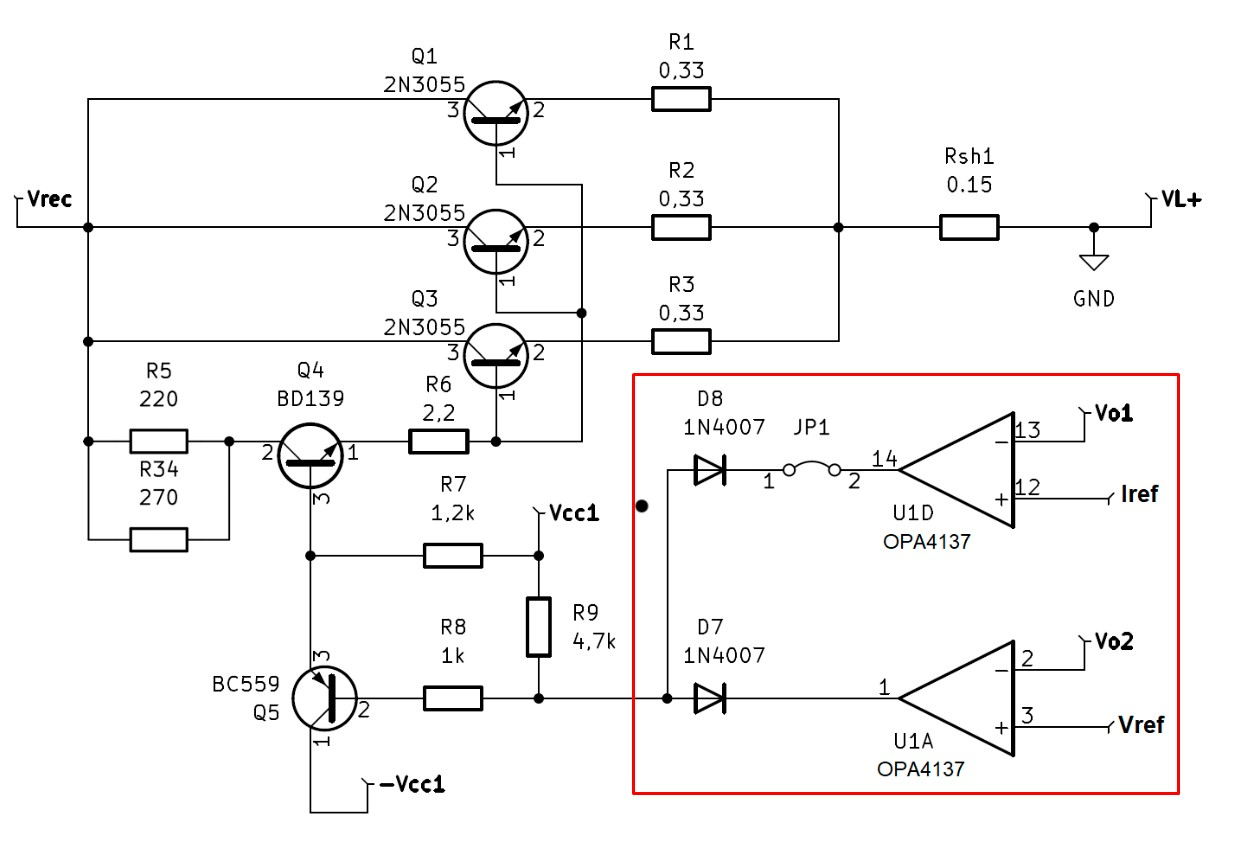
\includegraphics[scale=0.3]{./imagenes/Eliminada1.jpg}
    \caption{Sección de referencia de tensión.}
    \label{F:estructura_archivos}
\end{figure}

\subsection{Modificación de uso de Potenciómetros Digitales MCP4661}
Originalmente, los potenciómetros digitales MCP4661 se utilizaban para establecer una referencia de voltaje que comandaba los transistores, definiendo tanto la tensión como la corriente sobre la carga. Sin embargo, con la incorporación del DAC, esta función ya no es necesaria. En su lugar, los potenciómetros digitales ahora se utilizan para establecer una referencia de tensión destinada a un circuito de protección analógica contra cortocircuitos. Esta reasignación permite una respuesta inmediata para proteger la carga, evitando los retrasos inherentes a los cálculos y actualizaciones de salida necesarios en un sistema de control digital.
\begin{figure}[H]
    \centering
    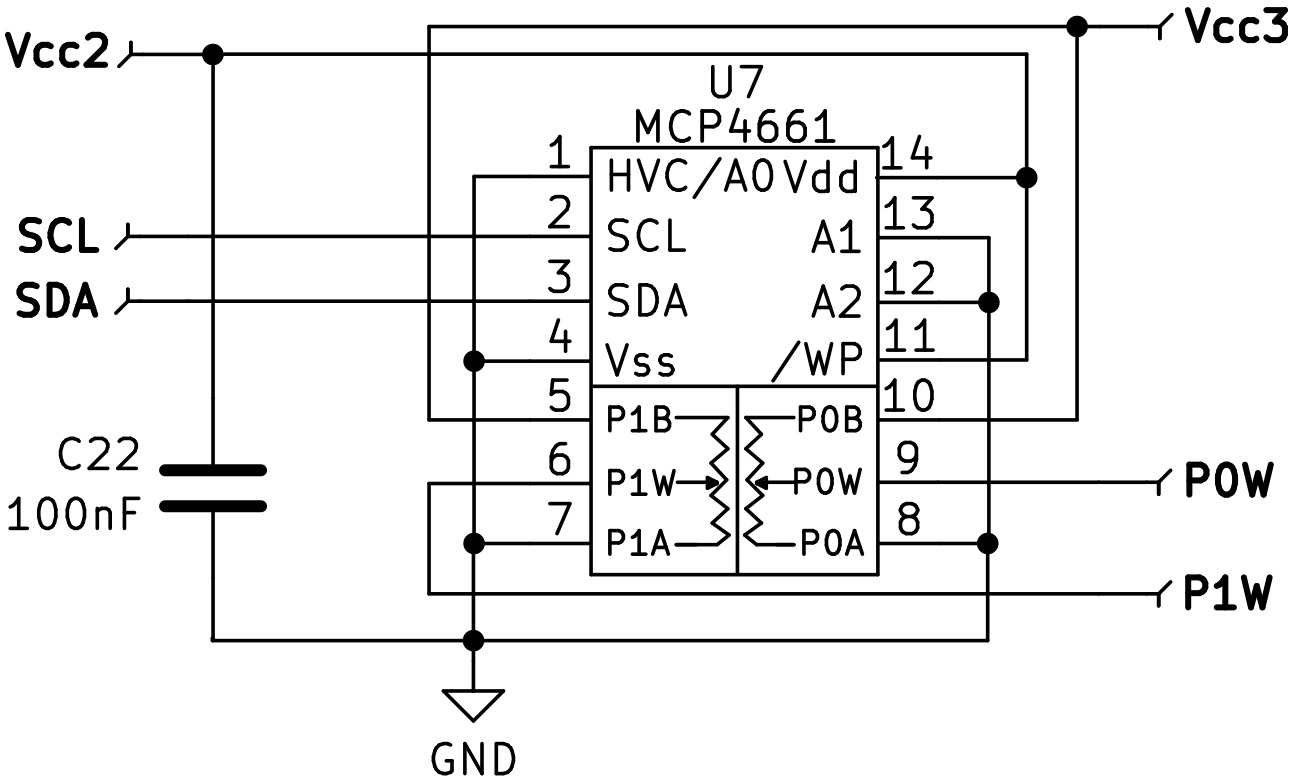
\includegraphics[scale=0.2]{./imagenes/potenciometro_digital.jpg}
    \caption{Potenciómetros digital MCP4661.}
    \label{F:potenciometro_digital}
\end{figure}

\subsection{Eliminación del circuito de medición externo}
Dado que la fuente de alimentación ahora cuenta con una pantalla integrada que muestra en tiempo real los valores de tensión y corriente, el circuito dedicado a la conexión de un voltímetro-amperímetro digital se ha considerado innecesario y, por lo tanto, ha sido eliminado. Esta simplificación reduce la complejidad del diseño y el número de componentes necesarios reduciendo los costos constructivos de la fuente.
\begin{figure}[H]
    \centering
    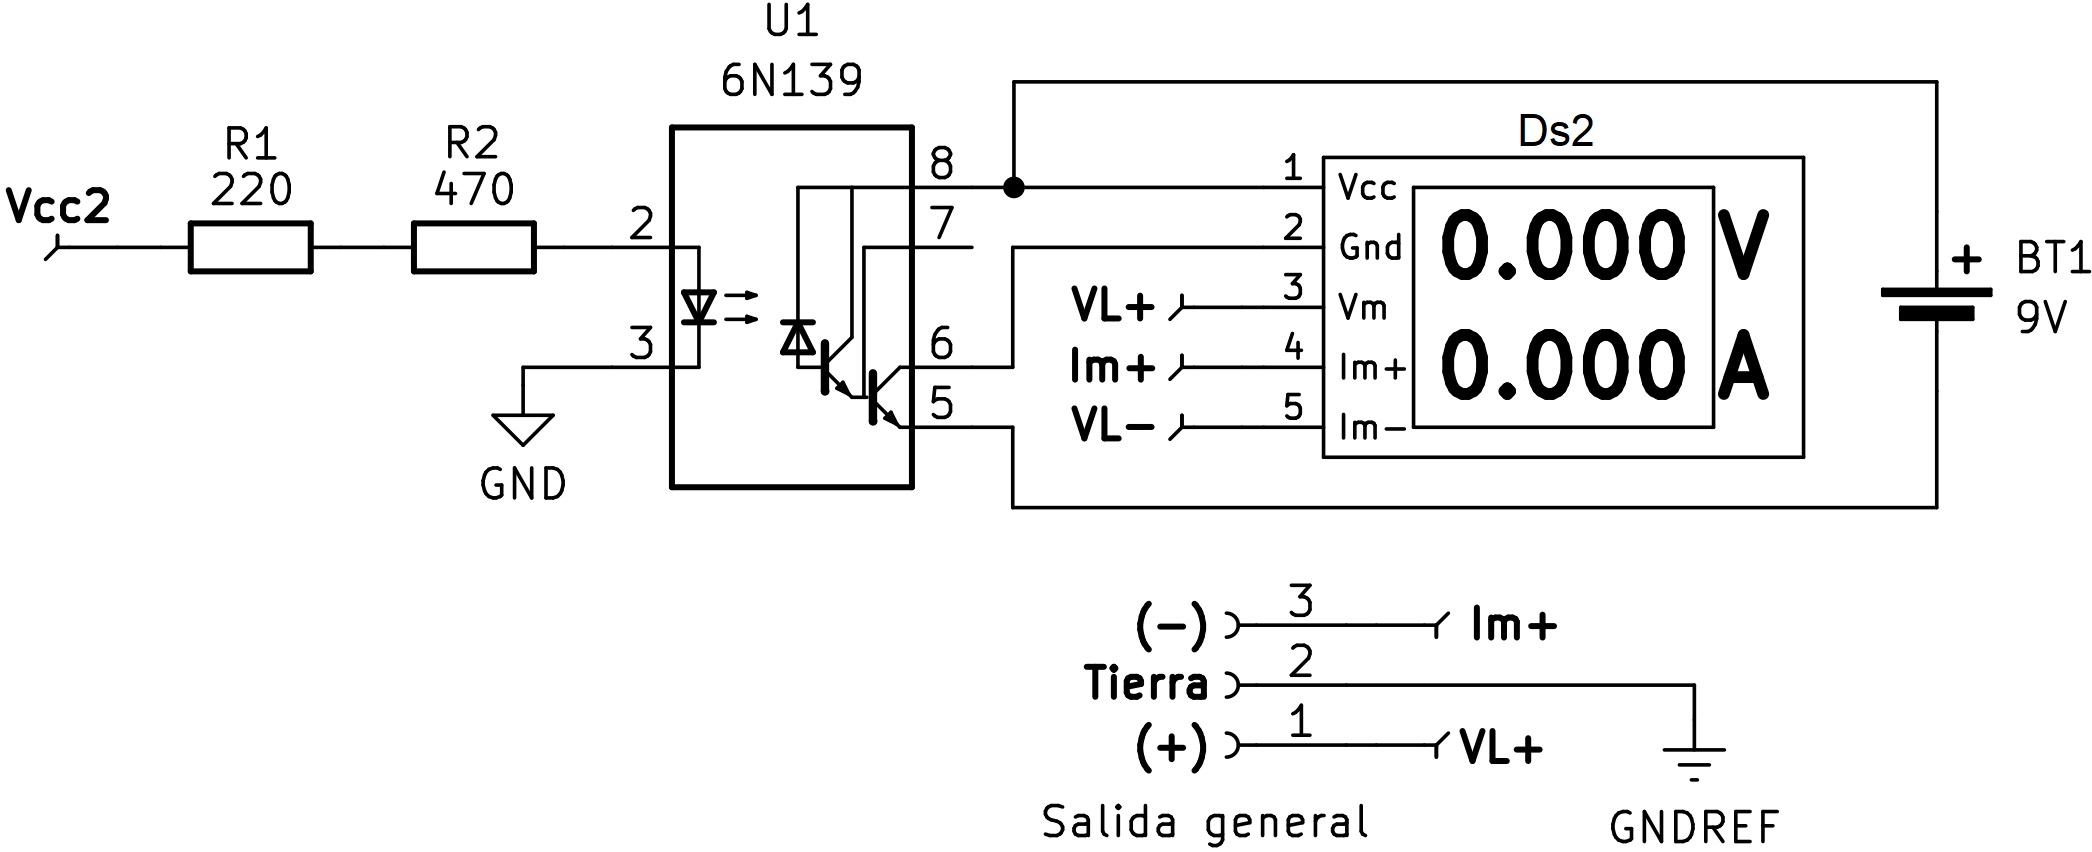
\includegraphics[scale=0.2]{./imagenes/voltimetro_amperimetro.jpg}
    \caption{Conexión voltímetro/amerimetro.}
    \label{F:voltimetro_amperimetro}
\end{figure}

\subsection{Modificación del Circuito de Acople y Desacople de Carga}
Se ha reducido considerablemente el circuito de disparo del optoacoplador, aprovechando las capacidades proporcionadas por el Arduino Nano para establecer un pin en estado alto.
\begin{figure}[H]
    \centering
    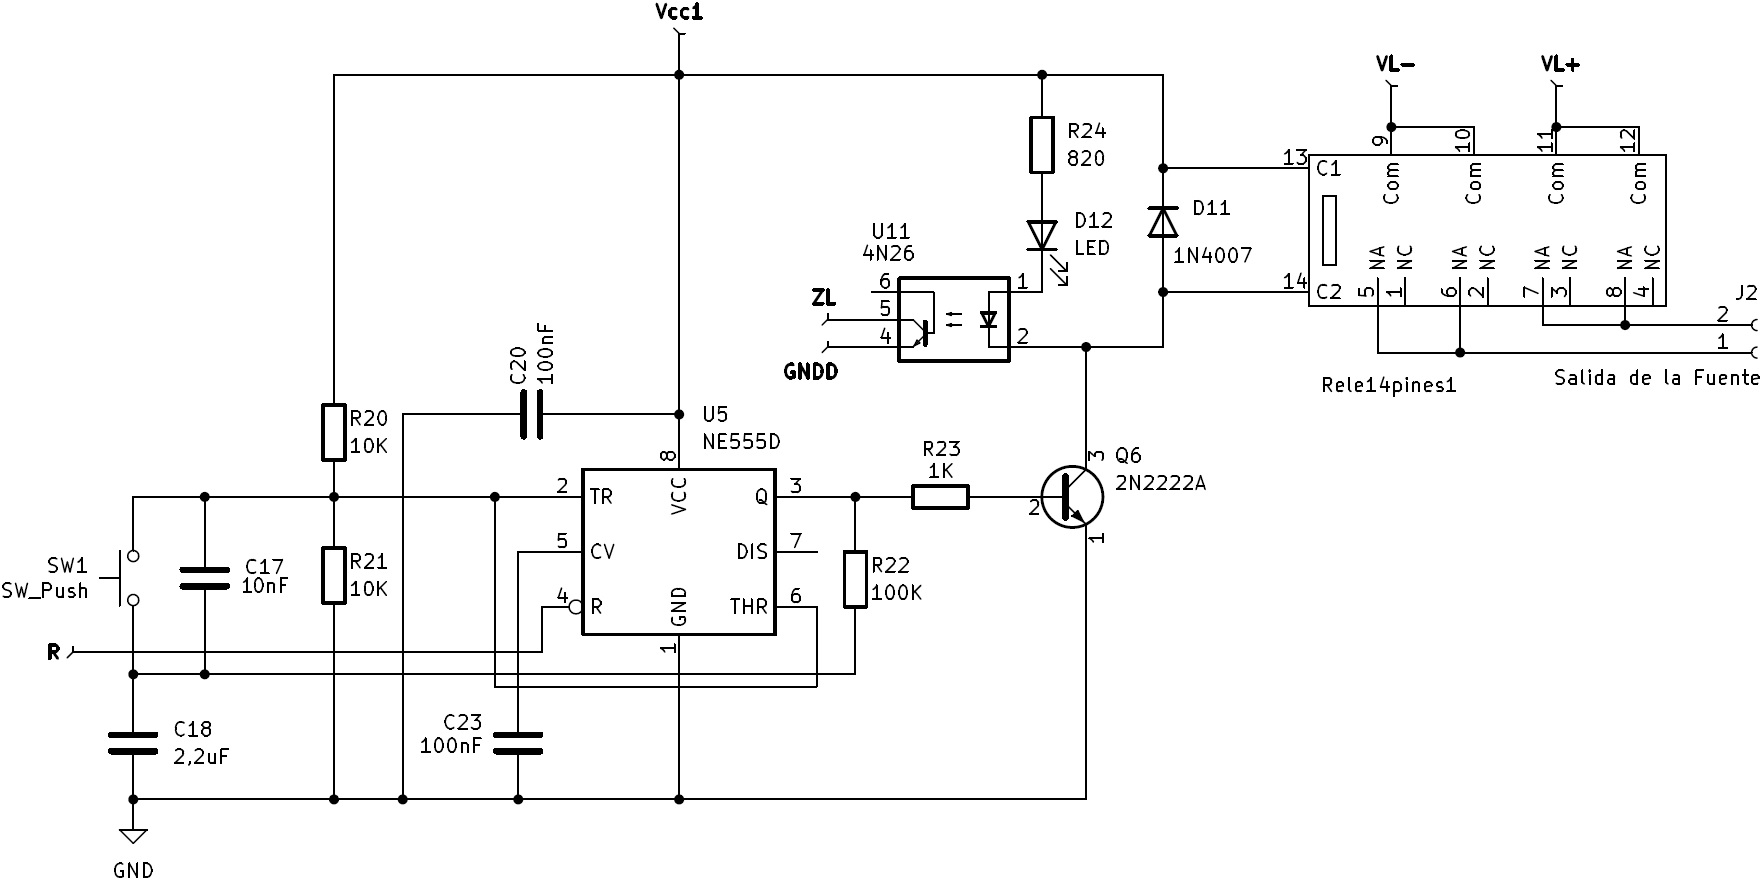
\includegraphics[scale=0.3]{./imagenes/conexion_carga.jpg}
    \caption{Acople y desacople de carga.}
    \label{F:conexion_carga}
\end{figure}

\subsection{Simplificación del Circuito Indicador de Modo de Operación}
La pantalla integrada también cumple la función de indicar el modo de operación, eliminando la necesidad de un circuito adicional dedicado a esta tarea. Esto no solo simplifica el diseño del sistema, sino que también mejora la usabilidad al centralizar toda la información relevante en un solo lugar.
\begin{figure}[H]
    \centering
    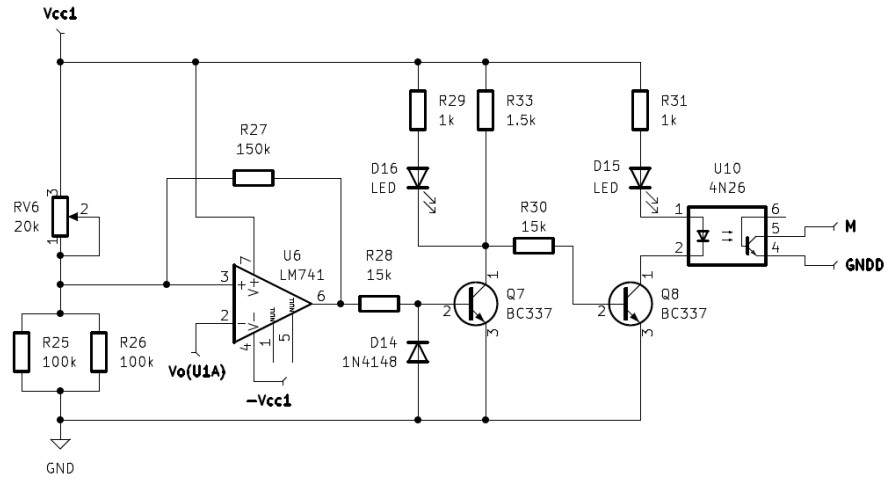
\includegraphics[scale=0.5]{./imagenes/modo_operacion.jpg}
    \caption{Sección de referencia de tensión.}
    \label{F:modo_operacion}
\end{figure}

\subsection{Integración del Circuito con NodeMCU ESP-32S}
Dado que no se requiere una conexión inalámbrica según las especificaciones del circuito, se ha prescindido del microcontrolador ESP con módulo Wi-Fi para visualizar la información en una computadora.
\begin{figure}[H]
    \centering
    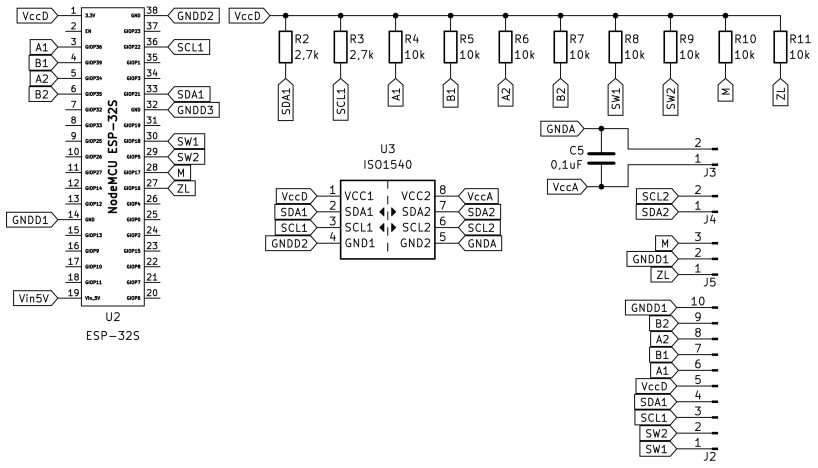
\includegraphics[scale=0.5]{./imagenes/ESP_32S.jpg}
    \caption{Circuito registrador de datos.}
    \label{F:ESP_32S}
\end{figure}

\subsection{Encoders rotativos}
El uso de un teclado numérico hace que este elemento se vuelva totalmente innecesario para estas aplicaciones dado a que el objetivo de la fuente es que sea totalmente digital evitando el ajuste manual de las magnitudes. Sin embargo no habría problema en implementar este elemento en paralelo en caso de un nuevo diseño para seteo de magnitudes, esto debido a una cuestión tradicional ya que la gran mayoría de los usuarios estan acostumbrado a setear manualmente las fuentes de tensión. 
\begin{figure}[H]
    \centering
    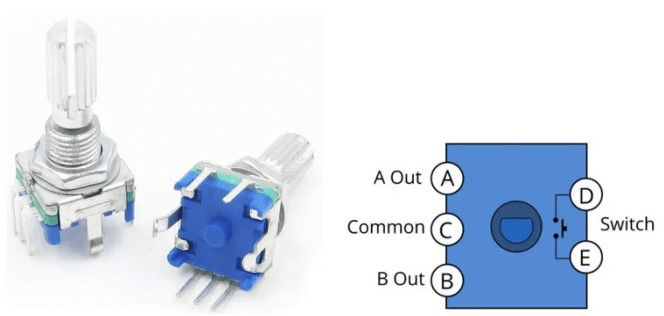
\includegraphics[scale=0.5]{./imagenes/encoder_rotativo.jpg}
    \caption{Encoder rotativos.}
    \label{F:encoder_rotativo}
\end{figure}

Estas modificaciones han permitido no solo modernizar la fuente de alimentación, sino también mejorar su funcionalidad y eficiencia mediante la incorporación de tecnología digital y la simplificación de circuitos redundantes. En las secciones siguientes, se detallarán en profundidad cada uno de estos cambios y su impacto en el rendimiento general del equipo






% ----------------------
  \chapter{Uso de esta plantilla en \LaTeX}

En este capítulo, en gran parte, se demostrará con ejemplos el uso de esta plantilla, y en general el uso de \LaTeX. Algunas cosas, como la estructura de archivos de esta plantilla, requieren cierta explicación, pero siempre que pueda evitarse, simplemente se utilizará un ejemplo de código y el resultado del compilado del mismo. \cite{Instruments1978}

Las cuestiones básicas sobre el uso de \LaTeX, más bien que ser explicadas de forma tediosa en este texto, se recomienda al alumno buscar videotutoriales en línea. Como ejemplo considere esta lista de reproducción \cite{tutorial_latex}.

La forma en la que se encuentra desarrollado este capítulo es sencillo y no requiere mayor explicación que la recién brindada.

% ----------------------
\section{Estructura del Informe}

En la figura~\ref{F:estructura_archivos} se puede ver la estructura de archivos. En la carpeta \entreComillas{contenido}, se encuentran los archivos que componen cada capítulo del informe; en \entreComillas{apéndices}, se encuentran los apéndices; en \entreComillas{imagenes}, las imágenes y gráficos utilizados, sea el formato que sea, \texttt{.png}, \texttt{.jpg}, \texttt{.pdf}, o cualquier otro; en \entreComillas{bibliografia} se encuentra el archivo \texttt{bibliografia.bib}, donde están especificadas todas las referencias utilizadas en el informe; y en \entreComillas{codigo}, se encuentra el código fuente de programas que se hayan incluido al informe.

Luego se tienen otros archivos que están fuera de las carpetas. Uno de ellos es el documento \texttt{proyectoelectronico.cls}, el cual es una clase donde se define el estilo de la plantilla; y el otro es \texttt{proyecto.tex}, el cual es el documento principal, el cual se compila para generar el archivo \texttt{.pdf} del informe.

\clearpage
\begin{figure}
    \centering
    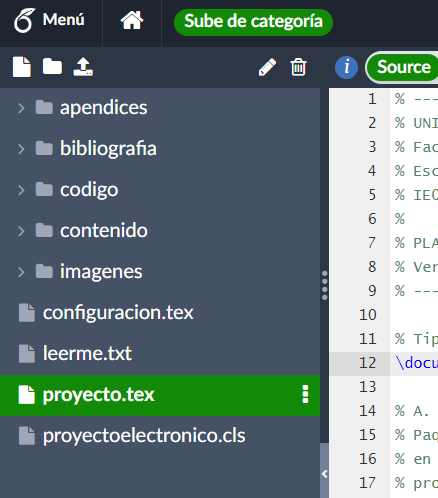
\includegraphics[scale=0.8]{./imagenes/estructura_de_archivos.png}
    \caption{Estructura de archivos de la plantilla.}
    \label{F:estructura_archivos}
\end{figure}



\clearpage
\subsection{Datos generales}

Los datos de la portada y la página de aprobación se ingresan en \texttt{proyecto.tex}. A continuación, se muestra exactamente donde se deben ingresar los datos.

\footnotesize
\begin{lstlisting}[language=TeX, numbers=none]
% Titulo del proyecto
\titulo{Colocar aqui el nombre del proyecto}

% Autor (nombre y carne)
\autoruno{Nombre del primer integrante}
\carneuno{Legajo del primer integrante} % legajo
\emailuno{Email del primer integrante}

\autordos{Nombre del segundo integrante}
\carnedos{Legajo del segundo integrante} % legajo
\emaildos{Email del segundo integrante}

%\autortres{Nombre del tercer integrante}
%\carnetres{Legajo del tercer integrante} % legajo
%\emailtres{Email del tercer integrante}

% Profesor(a) guia
\guia{Nombre del profesor tutor}

% Profesores lectores 
\lectorA{Nombre del primer profesor lector}
\lectorB{Nombre del segundo profesor lector}

% Fecha de entrega del trabajo escrito
\mes{11}	% Numero del mes
\ano{2022}	% Formato AAAA
\end{lstlisting}
\normalsize

Como puede apreciarse existen campos para incluir un tercer integrante al grupo, en caso de ser necesario, descomentar los campos y rellenarlos. Para poder visualizar al tercer integrante en la carátula, página de aprobación, resumen y abstract, debemos dirigirnos a \texttt{proyectoelectronico.cls} y descomentar algunas líneas; las mismas se muestran a continuación. Se recomienda utilizar el buscador (Ctrl + F) para encontrarlas rápidamente.

Estas líneas son de la carátula, y deben ser descomentadas si esperamos que el tercer integrante aparezca en la misma.

\footnotesize
\begin{lstlisting}[language=TeX, numbers=none]
%	\vskip 0.8em
%	\large\bfseries \@autortres \\
%	\vskip 0.1em
%	\large\bfseries \@emailtres \\
\end{lstlisting}
\normalsize

\clearpage
Estas líneas son de la hoja de aprobación, y deben ser descomentadas si esperamos que el tercer integrante aparezca en la misma.

\footnotesize
\begin{lstlisting}[language=TeX, numbers=none]
%	\large\bfseries \@autortres \\
%	\vskip 0.1em
%	\large\bfseries \@emailtres \\
%	\vskip 0.1em
%	\large\bfseries \@carnetres \\
\end{lstlisting}
\normalsize

Esta última línea se repite dos veces, una para el resumen y otra vez para el abstract. La misma debe ser descomentada en ambas partes si esperamos que el tercer integrante aparezca correctamente en ellas.

\footnotesize
\begin{lstlisting}[language=TeX, numbers=none]
%		\large\bfseries\@autortres
\end{lstlisting}
\normalsize

\subsection{Resumen}

Para escribir el resumen\footnote{Recordar que el resumen es una de las cosas que se termina por último, hay que tener el informe escrito casi en su totalidad para saber que escribir en el resumen. En esta sección simplemente se describe como modificarlo, pero debe realizarse por último.} es necesario ir al archivo \texttt{./contenido/resumen.tex}. El contenido actual del mismo se muestra a continuación.
\footnotesize
\begin{lstlisting}[language=TeX]
% EL RESUMEN
% ----------

\begin{resumen}{Aqui, van, las, palabras, claves, separadas, por, comas}

\lipsum[1-2]

\end{resumen}
\end{lstlisting}
\normalsize

Aquí debe agregarse las palabras claves separadas por coma, y luego escribir el resumen en sí. Para ello es necesario eliminar la línea con el comando \texttt{$\backslash$lipsum[1-2]}, el mismo es simplemente un comando para generar texto aleatorio con el objetivo de rellenar plantillas y ver como quedarían si tuviesen texto, por lo tanto, debe eliminarse antes de escribir el resumen.

\clearpage
\subsection{Abstract}

El abstract es simplemente una traducción del resumen y para escribirlo es necesario ir al archivo \texttt{./contenido/abstract.tex}. El contenido actual del mismo se muestra a continuación.
\footnotesize
\begin{lstlisting}[language=TeX]
% EL RESUMEN EN INGLES
% --------------------

\begin{theabstract} {Here goes the translated title of the project} {Here, goes, the, keywords, separated, by, commas}

\lipsum[1-2]

\end{theabstract}
\end{lstlisting}
\normalsize

Su modificación es similar a la del resumen, con la diferencia de que aquí el entorno \entreComillas{theabstract} recibe dos parámetros, primero el título traducido y luego las palabras claves, por supuesto, también en inglés.

Al igual que el resumen, para escribir el abstract es necesario eliminar la línea con el comando \texttt{$\backslash$lipsum[1-2]} antes.

\subsection{Agradecimientos}

Para agregar los agradecimientos es necesario simplemente modificar el archivo: \\ \texttt{./contenido/agradecimientos.tex}.

\subsection{Nomenclatura}

Para modificar las nomenclaturas utilizadas debe modificarse el archivo: \\ \texttt{./contenido/nomenclatura.tex}.

Para ello se utiliza el comando \texttt{$\backslash$nomenclature\{\}\{\}}, el mismo recibe dos parámetros, el primero de ellos es la abreviatura o palabra, y el segundo su significado. En el archivo actual se encuentran muchos ejemplos, los cuales deben ser quitados si no son utilizados y agregar los que sí aplican al informe.

\subsection{Índices}

En el archivo \texttt{proyecto.tex} se encuentra especificado cómo se imprime la tabla de contenidos

\footnotesize
\begin{lstlisting}[language=TeX, numbers=none]
% 5. TABLAS DE CONTENIDO, FIGURAS Y TABLAS
\tableofcontents
\listoffigures
\listoffotos
\listoftables
\lstlistoflistings
\end{lstlisting}
\normalsize

Como hay muchos índices separados, deberíamos retirar los que no utilizamos. Por ejemplo, si no incluimos el código de ningún programa, deberíamos no incluir el índice de listados, es decir, quitar el comando \texttt{$\backslash$lstlistoflistings}.

\clearpage
\subsection{Modificaciones extras}

La idea de utilizar una plantilla es precisamente poder simplemente escribir el documento sin tener que molestarse con los detalles de formateo del mismo. Sin embargo, si es de interés para el alumno realizar modificaciones, mencionamos que en el archivo \texttt{proyectoelectronico.cls} se encuentra formateado la portada:

\footnotesize
\begin{lstlisting}[language=TeX, numbers=none]
% 1. Formato de portada
% ---------------------

\newcommand{\portada}{
...
}
\end{lstlisting}
\normalsize

La hoja de aprobación:

\footnotesize
\begin{lstlisting}[language=TeX, numbers=none]
% 2. Formato de la hoja de aprobacion
% -----------------------------------

\newcommand{\aprobacion}{
...
}
\end{lstlisting}
\normalsize

El resumen:

\footnotesize
\begin{lstlisting}[language=TeX, numbers=none]
% 3. Formato del resumen
% ----------------------

\NewDocumentEnvironment{resumen}{ m }
{
...
}
\end{lstlisting}
\normalsize

El abstract:

\footnotesize
\begin{lstlisting}[language=TeX, numbers=none]
% 4. Formato del abstract
% -----------------------

\NewDocumentEnvironment{theabstract}{ m m }
{
...
}
\end{lstlisting}
\normalsize

La hoja de agradecimientos (llamado reconocimientos en el código):

\footnotesize
\begin{lstlisting}[language=TeX, numbers=none]
% 5. Formato de los reconocimientos
% ---------------------------------

\NewDocumentEnvironment{reconocimiento}{ m }
{
...
}
\end{lstlisting}
\normalsize


\clearpage
\subsection{Agregar un capítulo}

Para agregar un capítulo nuevo creamos un archivo dentro de la carpeta \texttt{./contenido/} haciendo click derecho y seleccionando \entreComillas{Archivo nuevo}, como puede apreciarse en la figura~\ref{F:crear_nuevo_capitulo}.

\begin{figure}[ht]
  \centering
  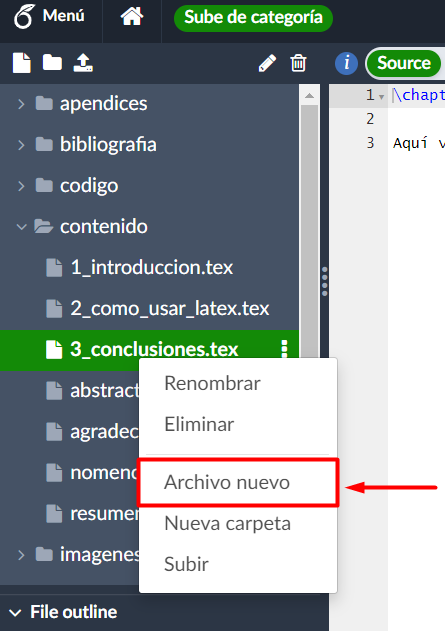
\includegraphics[width=0.45\textwidth]{./imagenes/crear_nuevo_capitulo.png}
  \caption{Creación de nuevo capítulo}
  \label{F:crear_nuevo_capitulo}
\end{figure}

Le asignamos al archivo un nombre apropiado y dentro del mismo utilizamos  \texttt{$\backslash$chapter\{\}}, para definir el capítulo y su nombre.

\footnotesize
\begin{lstlisting}[language=TeX, numbers=none]
\chapter{Nombre del nuevo capitulo}

% Texto de mi nuevo capitulo...
\end{lstlisting}
\normalsize

Dentro de este archivo es donde escribiremos nuestro capítulo. Pero para incluirlo al informe primero debemos dirigirnos al archivo \texttt{proyecto.tex}, y agregarlo con el comando \texttt{$\backslash$input\{\}}, teniendo en cuenta la posición del mismo respecto de los otros capítulos. Como puede observarse en la captura de la figura~\ref{F:nuevo_capitulo}, el mismo se agregó justo seguido de las conclusiones, pero podría ser puesto en otro orden.
\clearpage
\begin{figure}[ht]
  \centering
  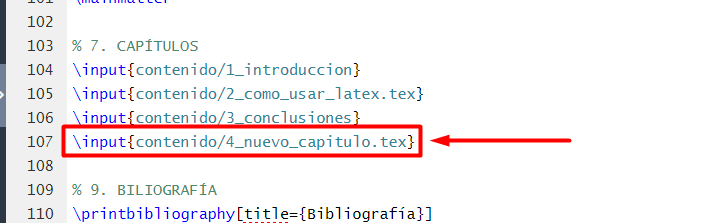
\includegraphics[width=0.85\textwidth]{./imagenes/nuevo_capitulo.png}
  \caption{Creación de nuevo capítulo}
  \label{F:nuevo_capitulo}
\end{figure}

\clearpage
\section{Figuras}

\footnotesize
\begin{lstlisting}
En la figura~\ref{F:diag_bloq_sistema_minimo} puede observarse el diagrama de bloques del sistema minimo.

\begin{figure}[ht]
  \centering
  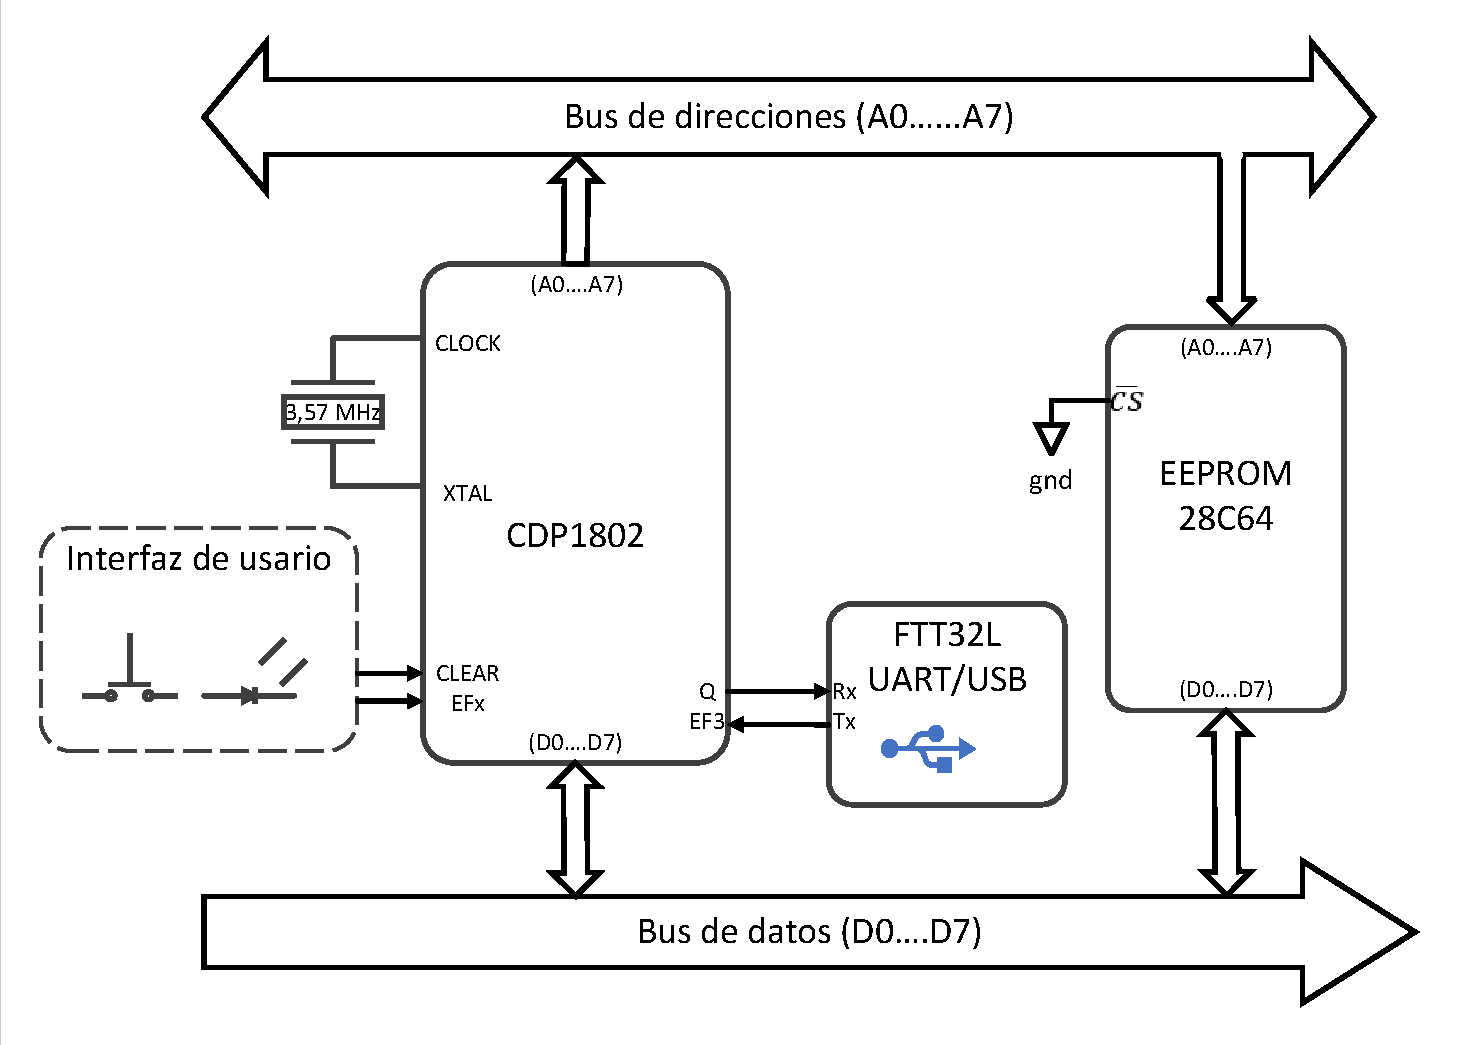
\includegraphics[width=0.9\textwidth]{./imagenes/diag_bloq_sistema_minimo.pdf}
  \caption{Diagrama de bloques del sistema minimo}
  \label{F:diag_bloq_sistema_minimo}
\end{figure}
\end{lstlisting}
\normalsize

En la figura~\ref{F:diag_bloq_sistema_minimo} puede observarse el diagrama de bloques del sistema mínimo.

\begin{figure}[ht]
  \centering
  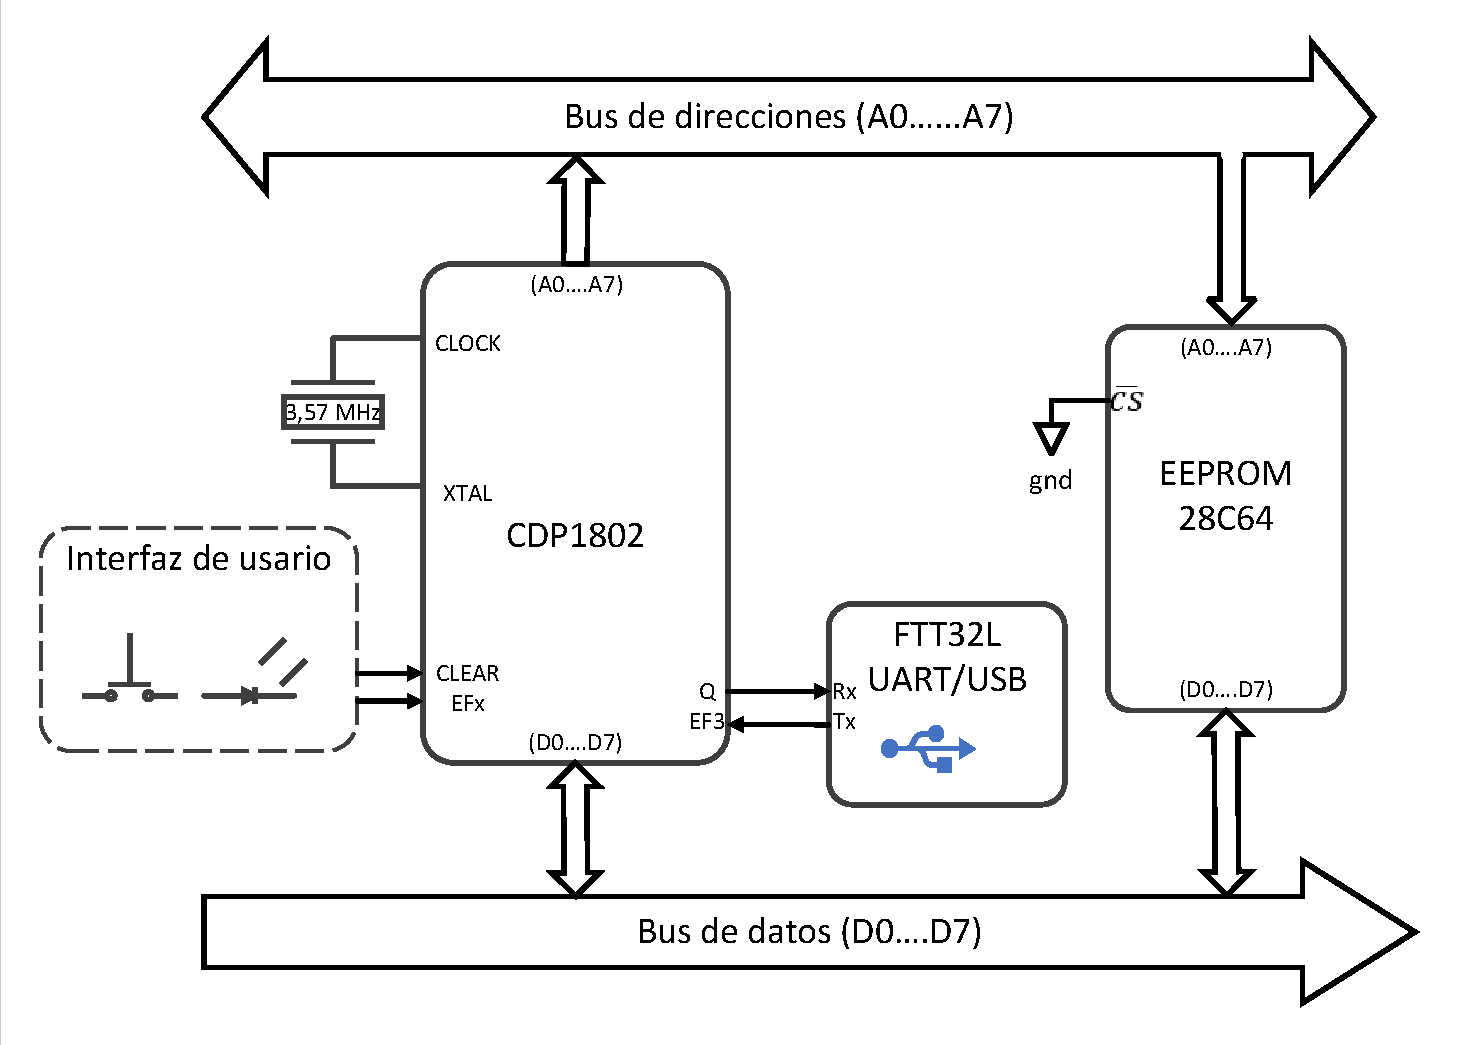
\includegraphics[width=0.9\textwidth]{./imagenes/diag_bloq_sistema_minimo.pdf}
  \caption{Diagrama de bloques del sistema mínimo}
  \label{F:diag_bloq_sistema_minimo}
\end{figure}

\clearpage
\footnotesize
\begin{lstlisting}
\begin{figure}[ht!]
\centering
\subfloat[Transistor (texto que aparece en el indice)][Transistor en encapsulado TO-220]{
	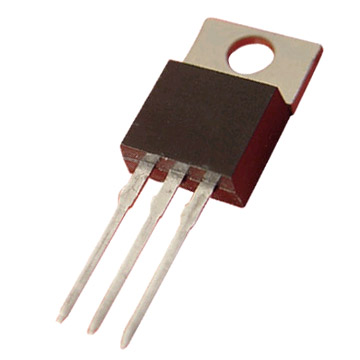
\includegraphics[width=0.2\textwidth]{./imagenes/transistor.jpg}
	\label{F:subfig1}}
\qquad
\subfloat[LED][LED blanco de baja potencia]{
	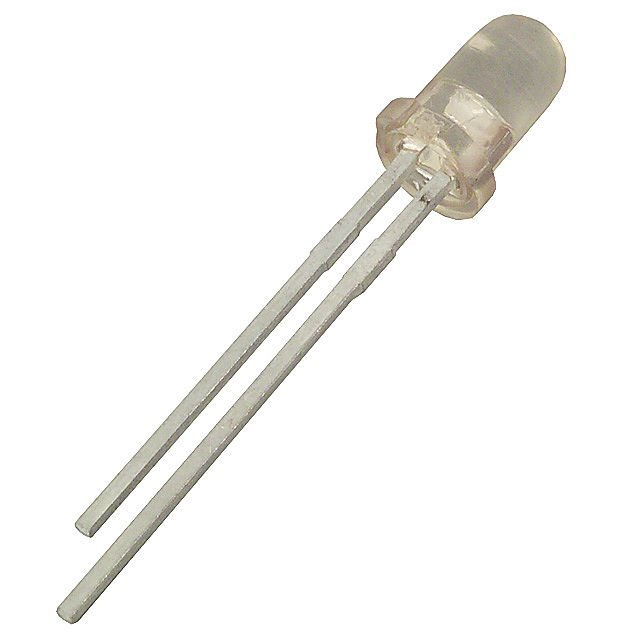
\includegraphics[width=0.2\textwidth]{./imagenes/led.jpg}
	\label{F:subfig2}}
\\
\subfloat[Fotoconductor][Fotoconductor]{
	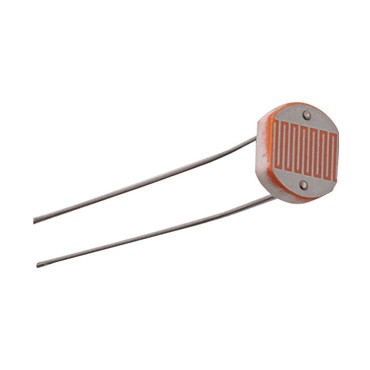
\includegraphics[width=0.2\textwidth]{./imagenes/fotoconductor.jpg}
	\label{F:subfig3}}
\qquad
\subfloat[Circuito integrado][Circuito integrado en encapsulado DIP-8]{
	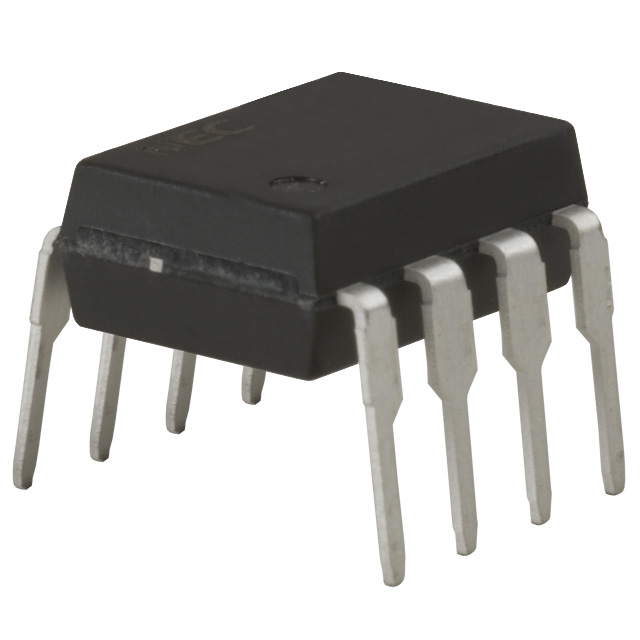
\includegraphics[width=0.2\textwidth]{./imagenes/integrado.jpg}
	\label{F:subfig4}}
\caption{Una figura con varias subfiguras, utilizando el paquete \texttt{subfig}}
\label{F:subfiguras}
\end{figure}
\end{lstlisting}
\normalsize


\begin{figure}[ht!]
\centering
\subfloat[Transistor (texto que aparece en el índice)][Transistor en encapsulado TO-220]{
	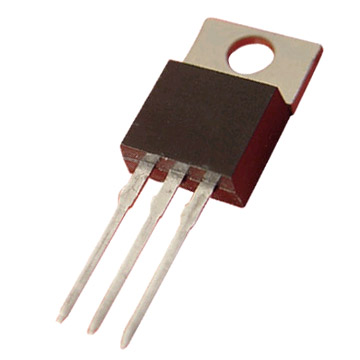
\includegraphics[width=0.2\textwidth]{./imagenes/transistor.jpg}
	\label{F:subfig1}}
\qquad
\subfloat[LED][LED blanco de baja potencia]{
	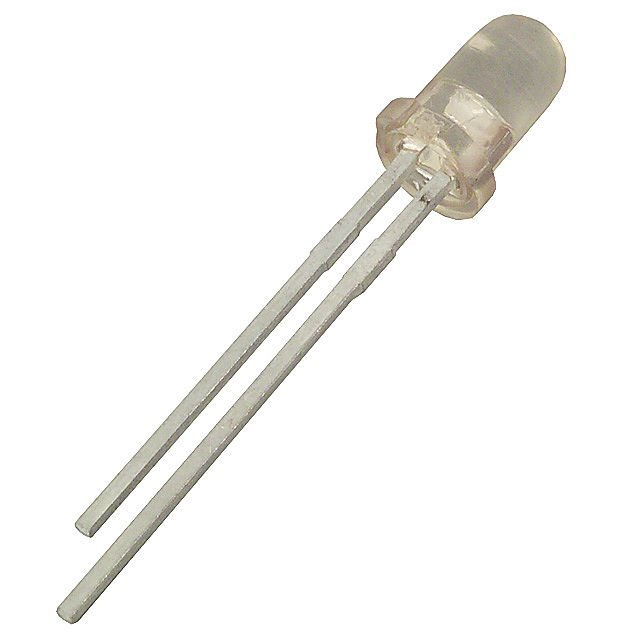
\includegraphics[width=0.2\textwidth]{./imagenes/led.jpg}
	\label{F:subfig2}}
\\
\subfloat[Fotoconductor][Fotoconductor]{
	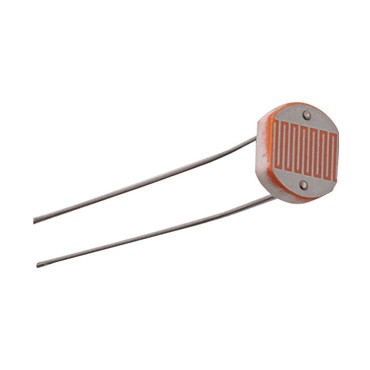
\includegraphics[width=0.2\textwidth]{./imagenes/fotoconductor.jpg}
	\label{F:subfig3}}
\qquad
\subfloat[Circuito integrado][Circuito integrado en encapsulado DIP-8]{
	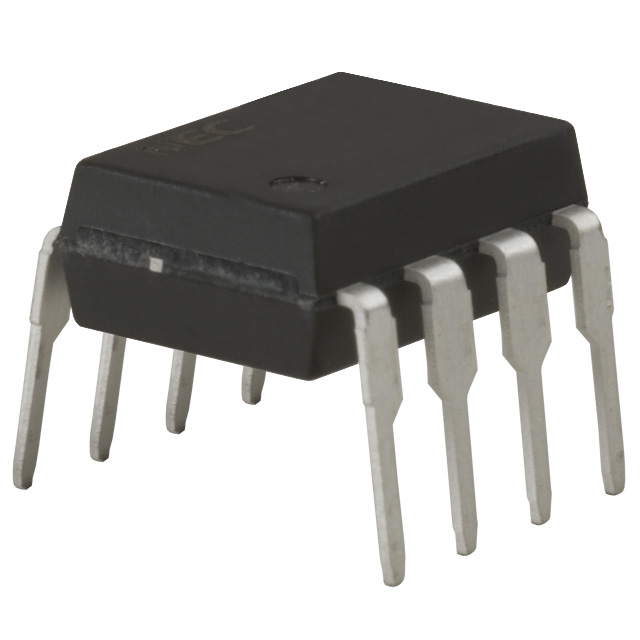
\includegraphics[width=0.2\textwidth]{./imagenes/integrado.jpg}
	\label{F:subfig4}}
\caption{Una figura con varias subfiguras, utilizando el paquete \texttt{subfig}}
\label{F:subfiguras}
\end{figure}

\clearpage
\section{Fotografías}

A pedido de la cátedra se incluyó un entorno distinto al de figuras para presentar fotografías. El mismo se utiliza de igual manera que el entorno de figuras, con la única diferencia de que este entorno se llama \entreComillas{foto}, como se muestra a continuación.

\footnotesize
\begin{lstlisting}
En la fotografia~\ref{F:foto_sistema_med} puede verse el sistema medio construido.

\begin{foto}[ht]
  \centering
  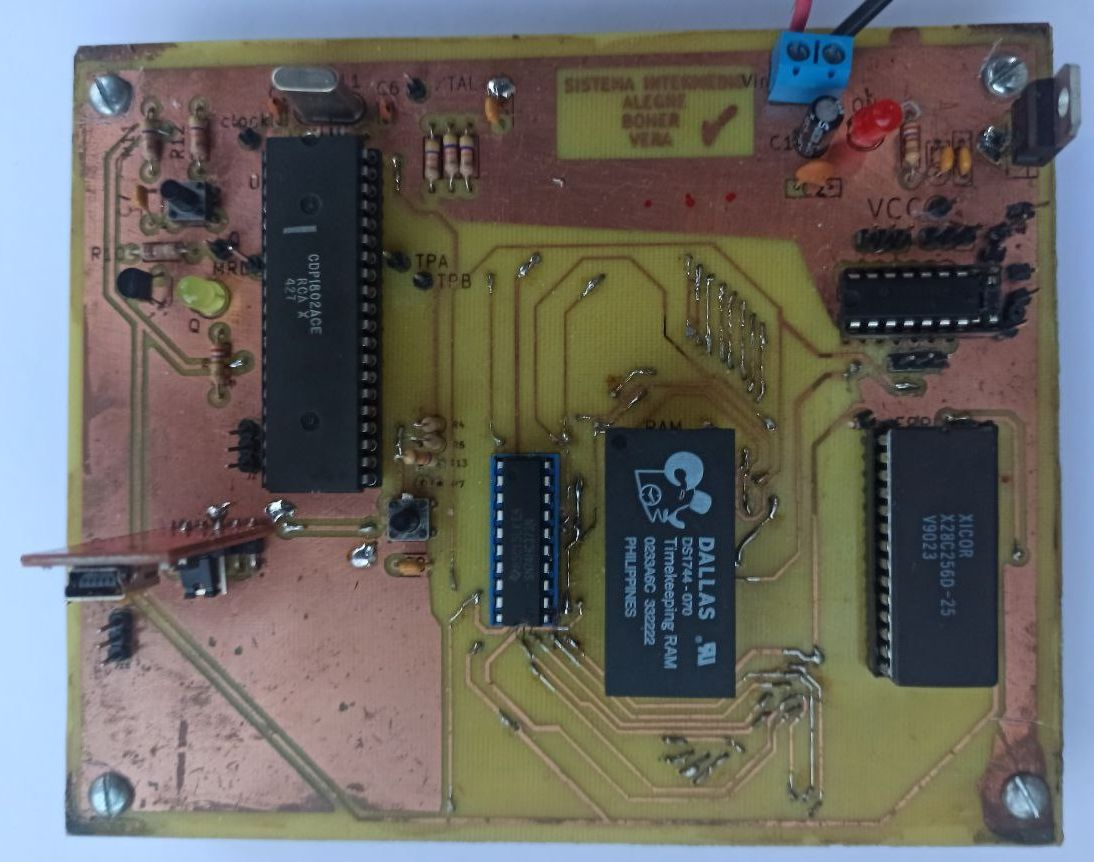
\includegraphics[width=0.9\textwidth]{./imagenes/foto_sistema_med.jpg}
  \caption{Sistema medio construido}
  \label{F:foto_sistema_med}
\end{foto}
\end{lstlisting}
\normalsize

En la fotografía~\ref{F:foto_sistema_med} puede verse el sistema medio construido.

\begin{foto}[ht]
  \centering
  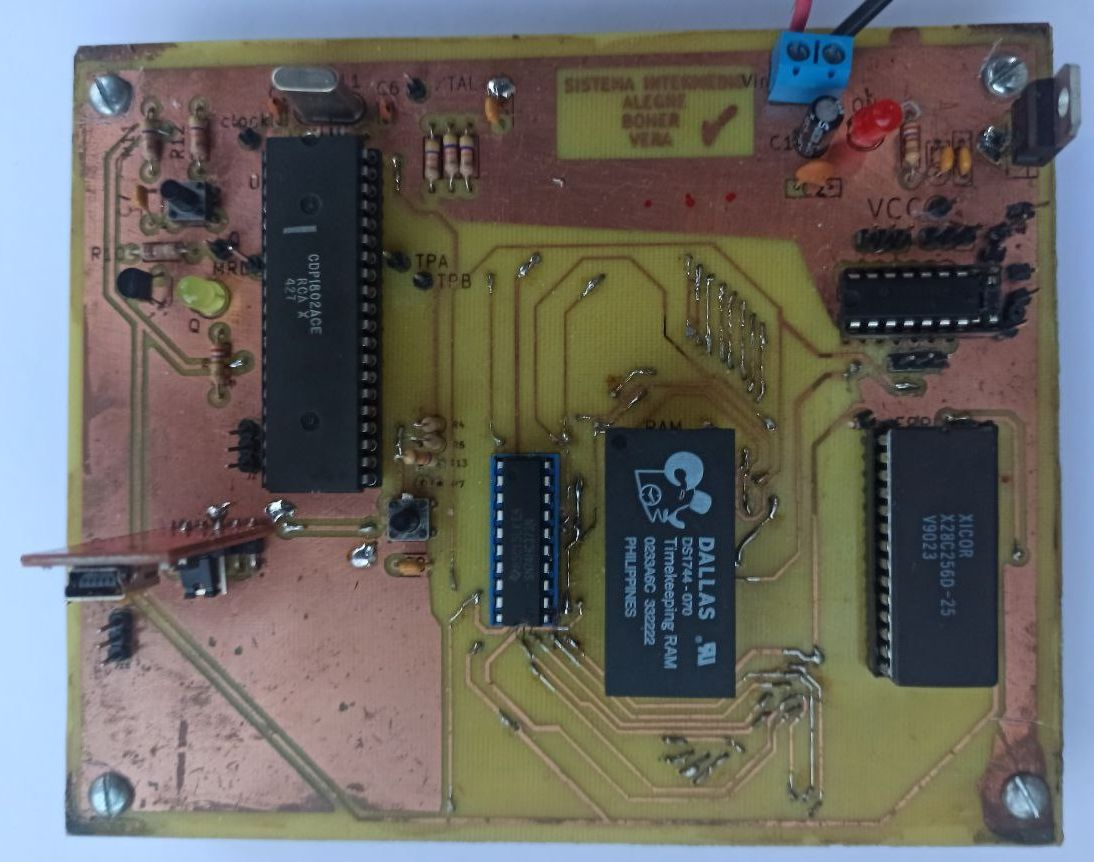
\includegraphics[width=0.9\textwidth]{./imagenes/foto_sistema_med.jpg}
  \caption{Sistema medio construido}
  \label{F:foto_sistema_med}
\end{foto}



\clearpage
\section{Tablas}

A continuación, se muestran algunas tablas como ejemplo. Existen páginas para crear tablas de \LaTeX~de forma rápida y sencilla, como por ejemplo \cite{tablas_latex_online}; el cual se utilizó en varias ocasiones.


\begin{table}[ht!]
\caption{Numeración decimal, binaria y hexadecimal}
\label{T:dec_bin_hex}
\begin{tabular}{|c|c|c|}
\hline
Decimal & Binario & Hexadecimal \\ \hline \hline
0       & 0000    & 0           \\ \hline
1       & 0001    & 1           \\ \hline
2       & 0010    & 2           \\ \hline
3       & 0011    & 3           \\ \hline
4       & 0100    & 4           \\ \hline
5       & 0101    & 5           \\ \hline
6       & 0110    & 6           \\ \hline
7       & 0111    & 7           \\ \hline
8       & 1000    & 8           \\ \hline
9       & 1001    & 9           \\ \hline
10      & 1010    & A           \\ \hline
11      & 1011    & B           \\ \hline
12      & 1100    & C           \\ \hline
13      & 1101    & D           \\ \hline
14      & 1110    & E           \\ \hline
15      & 1111    & F           \\ \hline
\end{tabular}
\end{table}


% Please add the following required packages to your document preamble:
% \usepackage{multirow}
\begin{table}[ht!]
\caption{Códigos de estado}
\label{T:state_codes}
\begin{tabular}{|l|ll|}
\hline
\multicolumn{1}{|c|}{\multirow{2}{*}{State Type}} & \multicolumn{2}{l|}{State Code} \\ \cline{2-3} 
\multicolumn{1}{|c|}{}                            & \multicolumn{1}{l|}{SC1}  & SC0 \\ \hline
S0 (Fetch)                                        & \multicolumn{1}{l|}{L}    & L   \\ \hline
S1 (Execute)                                      & \multicolumn{1}{l|}{L}    & H   \\ \hline
S2 (DMA)                                          & \multicolumn{1}{l|}{H}    & L   \\ \hline
S3 (Interrupt)                                    & \multicolumn{1}{l|}{H}    & H   \\ \hline
\end{tabular}
\end{table}


\clearpage

La tabla~\ref{T:bom_sis_final} es un ejemplo de cómo realizar una tabla que es tan grande que se extiende en varias páginas. La misma tiene un encabezado que se repite en cada página, de manera que no es necesario ir al comienzo de la tabla para ver a qué corresponde cada columna, dado que el encabezado está presente al inicio de cada página.

\footnotesize
\begin{longtable}{|P{0.08\textwidth}|P{0.11\textwidth}|P{0.30\textwidth}|P{0.14\textwidth}|P{0.15\textwidth}|}
\caption{Lista de componentes del sistema final} % needs to go inside longtable environment
\label{T:bom_sis_final}
\\
\hline
Cantidad & Etiqueta \newline
           Identificador            & Descripción                               & Fabricante            & Número de parte       \\ \hline \hline \endfirsthead
\hline
Cantidad & Etiqueta \newline
           Identificador            & Descripción                               & Fabricante            & Número de parte       \\ \hline \hline \endhead
1       & U1                        & Microprocesador                           & RCA                   & CDP1802ACE            \\ \hline
1       & U2                        & Latch de 8 bits                           & Philips               & 74HC573N              \\ \hline
1       & U3                        & Memoria EEPROM 32k x 8                    & XICOR                 & X28C256D-25           \\ \hline
1       & U4                        & Memoria EEPROM Serial I2C 128k x 8        & Microchip             & 24LC1025              \\ \hline
1       & U5                        & Time keeping RAM 32K x8                   & Dallas                & DS1744-070            \\ \hline
1       & U6                        & Memoria RAM 32k x 8                       & HYUNDAI               & HY62256ALP-10         \\ \hline
1       & U7                        & Memoria FRAM Serial I2C 8k x 8            & Fujitsu Semiconductors & MB85RC64A            \\ \hline
1       & U8                        & Conversor analógico-digital con interfaz I2C & Maxim Integrated   & MAX127                \\ \hline
1       & U9                        & Regulador de tensión 12~\si{\volt}        & Motorola              & 7812CT                \\ \hline
1       & U10                       & Regulador de tensión 5~\si{\volt}         & ST Microelectronics   & L7805CV               \\ \hline
1       & U11                       & High Precision Operational Amplifier      & Burr Brown            & OPA4277PA             \\ \hline
1       & U12                       & Regulador de tensión -12~\si{\volt}       & ST Microelectronics   & L7912CV               \\ \hline
5       & U13, U14, U15, U16, U28   & Cuadruple compuerta NAND de dos entradas  & Texas Instrument      & SN74HC00N             \\ \hline
1       & U17                       & Cuadruple compuerta NAND de dos entradas con Schmitt-Trigger & Texas Instrument & SN74HC132N \\ \hline
2       & U18,U30                   & Cuadruple compuerta NOR de dos entradas   & Texas Instrument      & SN74HC02N             \\ \hline
1       & U19                       & Decodificador Multiplexador 3 a 8 líneas  & Texas Instrument      & SN74HC138N            \\ \hline
1       & U20                       & CMOS Programmable Peripheral Interface    & Intersil              & CP82C55A-5Z           \\ \hline
1       & U21                       & Regulador programable shunt               & Fairchild             & LM336Z25              \\ \hline
1       & U24                       & Doble flip-flop tipo D con Set y Reset    & Texas Instrument      & SN74HC74N             \\ \hline
1       & U25                       & Contador binario de 4 bits                & Fairchild Semiconductor & MM74HC161N          \\ \hline
1       & U29                       & Doble flip-flop JK con Set y Reset        & National Semiconductors & MM74HC73N           \\ \hline
1       & U31                       & Registro de desplazamiento de 8 bits      & Texas Instrument      & SN74HC595N            \\ \hline
1       & U32                       & Registro de desplazamiento de 8 estados   & Motorola              & MC14014BCP            \\ \hline
1       & X2                        & XO-22BE-4MHz                              &   \listaVacio                    & \listaVacio                      \\ \hline
1       & XTAL1                     & Cristal \num{4}~\si{\mega\hertz}          & CQ Electronics        & \listaVacio                      \\ \hline
1       & SW1                       & Llave DPDT 6 pines                        & \listaVacio                      & \listaVacio                      \\ \hline
3       & SW2, SW3, SW4             & Pulsador 6mm~x~4,3mm                      &  \listaVacio                     &  \listaVacio                     \\ \hline
5       & T2, T3, T4, T5, T6        & Transistor BJT NPN                        & Motorola              & P2N2222A               \\ \hline
1       & RV1                       & Preset 10~\si{\kilo\ohm}                  &  \listaVacio                     &  \listaVacio                     \\ \hline
1       & D1                        & Puente rectificador de onda completa B380R &            \listaVacio           &  \listaVacio                     \\ \hline
6       & D2, D3, D4, D5, D6, D7    & LED 5~mm                                  &\listaVacio                       &   \listaVacio                    \\ \hline
2       & D8, D9                    & 1N914                                     &\listaVacio                       &  \listaVacio                     \\ \hline
1       & F1                        & Fusible 10~mm 1~\si{\ampere}              &\listaVacio                       &  \listaVacio                     \\ \hline
8       & R1, R2, R3, R5, R21, R22, R23, R27
                                    & Resistor 47~\si{\kilo\ohm} 1/8~\si{\watt} & \listaVacio                      &   \listaVacio                    \\ \hline
1       & R4                        & Resistor 10~\si{\mega\ohm} 1/8~\si{\watt} &  \listaVacio                     &   \listaVacio                    \\ \hline
1       & R6                        & Resistor 330~\si{\ohm} 1/4~\si{\watt}     &  \listaVacio                     &   \listaVacio                    \\ \hline
2       & R7, R8                    & Resistor 1~\si{\kilo\ohm} 1/8~\si{\watt}  &  \listaVacio                     &    \listaVacio                   \\ \hline
3       & R9, R10, R11              & Resistor 220~\si{\ohm} 1/4~\si{\watt}     &    \listaVacio                   &    \listaVacio                   \\ \hline
16      & R12, R13, R14, R15, R16, R17, R18, R38, R39, R40, R41, R46, R47, R56, R57, R60
                                    & Resistor 10~\si{\kilo\ohm} 1/8~\si{\watt} & \listaVacio                      &   \listaVacio                    \\ \hline
5       & R19, R20, R24, R25, R26   & Resistor 100~\si{\kilo\ohm} 1/8~\si{\watt}&  \listaVacio                     &   \listaVacio                    \\ \hline
4       & R28, R30, R36, R52        & Resistor 100~\si{\ohm} 1/4~\si{\watt}     &  \listaVacio                     &   \listaVacio                    \\ \hline
4       & R29, R31, R37, R53        & Resistor 150~\si{\ohm} 1/4~\si{\watt}     &  \listaVacio                     &   \listaVacio                    \\ \hline
8       & R32, R33, R34, R35, R42, R43, R54, R55
                                    & Resistor 390~\si{\kilo\ohm} 1/8~\si{\watt}&  \listaVacio                     & \listaVacio                      \\ \hline
8       & R44, R45, R48, R49, R50, R51, R58, R59
                                    & Resistor 1~\si{\mega\ohm} 1/8~\si{\watt}  &  \listaVacio                     & \listaVacio                      \\ \hline
2       & C2, C3                    & Capacitor cerámico \num{30}~\si{\pico\farad} 50~\si{\volt}
                                                                                &   \listaVacio                    & \listaVacio                      \\ \hline
14       & C5, C7, C8, C29, C30, C31, C14, C15, C18, C32, C33, C39, C40, C43
                                    & Capacitor cerámico \num{0.10}~\si{\micro\farad} 50~\si{\volt}
                                                                                &    \listaVacio                   &   \listaVacio                    \\ \hline
1       & C11, C17                  & Capacitor electrolítico 4700~\si{\micro\farad} 25~\si{\volt}
                                                                                &     \listaVacio                  &   \listaVacio                    \\ \hline
2       & C12, C16                  & Capacitor cerámico \num{0.33}~\si{\micro\farad} 50~\si{\volt}
                                                                                &   \listaVacio                    &  \listaVacio                     \\ \hline
1       & C13                       & Capacitor electrolítico 10~\si{\micro\farad} 25~\si{\volt}
                                                                                &   \listaVacio                    &  \listaVacio                     \\ \hline
1       & C19                       & Capacitor electrolítico \num{0.01}~\si{\micro\farad} 25~\si{\volt}
                                                                                &     \listaVacio                  &  \listaVacio                     \\ \hline
1       & C20                       & Capacitor electrolítico \num{4.7}~\si{\micro\farad} 25~\si{\volt}
                                                                                &   \listaVacio                    &  \listaVacio                     \\ \hline
6       & J1, J2, J33, J48, J49, J50& 1x3 Pines Conectores Macho \num{2.54}~mm  &   \listaVacio                    &  \listaVacio                     \\ \hline
38      & J3, J4, J5, J6, J7, J8, J9, J10, J11, J12, J13, J14, J15, J16, J17, J18, J19, J20, J21, J22, J23, J24, J25, J26, J27, J28, J29, J30, J31, J36, J40, J41, J42, J45, J46, J51, J52, J53
                                    & Pin conector macho (1 \textit{Male Header Pin}) & \listaVacio                      &   \listaVacio                    \\ \hline
3       & J32, J35, J38             & 1x6 Pines Conectores Macho \num{2.54}~mm  & \listaVacio                      & \listaVacio                      \\ \hline
3       & J34, J37, J39             & 1x5 Pines Conectores Macho \num{2.54}~mm  & \listaVacio                      &   \listaVacio                    \\ \hline
2       & J43, J44                  & Bornera 3 pines \num{5.08}~mm             &  \listaVacio                     &  \listaVacio                     \\ \hline
2       & J47, J54                  & 1x12 Pines Conectores Macho \num{2.54}~mm &   \listaVacio                    &  \listaVacio                     \\ \hline
1       & J55                       & 1x2 Pines Conectores Macho \num{2.54}~mm  &   \listaVacio                    &   \listaVacio                    \\ \hline
1       & No aplica                 & Módulo conversor USB-Serial               & Future Technology Devices International & FT232RL \\ \hline
1       & No aplica                 & Módulo adaptador tarjeta micro SD         & \listaVacio  & \listaVacio \\ \hline
\end{longtable}
\normalsize

\clearpage
\section{Números y Unidades}

A continuación, se muestra como escribir unidades de forma correcta.


\begin{lstlisting}[language=TeX, numbers=none]
Las unidades se escriben utilizando el paquete siunitx. Puede ser asi: \SI{2.2}{\kilo\ohm}, o tambien ser asi: \num{2.2} \si{\kilo\ohm}.
\end{lstlisting}
\normalsize

Si compilamos esto, obtenemos:

Las unidades se escriben utilizando el paquete siunitx. Puede ser así: \SI{2.2}{\kilo\ohm}, o también ser así: \num{2.2} \si{\kilo\ohm}.

\vspace{1cm}

Pero es importante utilizar correctamente el espacio de no separación \textasciitilde~(que es el carácter 126 del código ASCII) para separar el número de la unidad, si se escriben por separado. De esta manera se evita que en los saltos de línea se separe el número de la unidad. Reescribamos lo anterior pero esta vez con un espacio de no separación.


\begin{lstlisting}[language=TeX, numbers=none]
Las unidades se escriben utilizando el paquete siunitx. Puede ser asi: \SI{2.2}{\kilo\ohm}, o tambien ser asi: \num{2.2}~\si{\kilo\ohm}.
\end{lstlisting}
\normalsize

Si compilamos esto, obtenemos:

Las unidades se escriben utilizando el paquete siunitx. Puede ser asi: \SI{2.2}{\kilo\ohm}, o tambien ser asi: \num{2.2}~\si{\kilo\ohm}.

\vspace{1cm}

Como vemos, ahora no se separó el número de la unidad.

\clearpage
\section{Ecuaciones}

\footnotesize
\begin{lstlisting}
En la ecuacion~\eqref{eq:ecuacion_1} se encuentra la formula de Euler.

\begin{equation}
\label{eq:ecuacion_1}
 e^{jx} = \cos{x} + j \sin{x}
\end{equation}
\end{lstlisting}
\normalsize

En la ecuación~\eqref{eq:ecuacion_1} se encuentra la fórmula de Euler.

\begin{equation}
\label{eq:ecuacion_1}
 e^{jx} = \cos{x} + j \sin{x}
\end{equation}

\footnotesize
\begin{lstlisting}
\begin{equation}
u(x) = 
  \begin{cases} 
   \exp{x} & \text{si } x \geq 0 \\
   1       & \text{si } x < 0
  \end{cases}
\end{equation}
\end{lstlisting}
\normalsize

\begin{equation}
u(x) = 
  \begin{cases} 
   \exp{x} & \text{si } x \geq 0 \\
   1       & \text{si } x < 0
  \end{cases}
\end{equation}

\footnotesize
\begin{lstlisting}
\begin{subequations}
    \begin{equation}
    r_1^2 = (h_T-h_R)^2+d^2
    \label{eq: r1_tierra_plana}
    \end{equation}
    \begin{equation}
    r_2^2 = (h_T+h_R)^2+d^2
    \label{eq: r2_tierra_plana}
    \end{equation}
\end{subequations}
\end{lstlisting}
\normalsize

\begin{subequations}
    \begin{equation}
    r_1^2 = (h_T-h_R)^2+d^2
    \label{eq: r1_tierra_plana}
    \end{equation}
    \begin{equation}
    r_2^2 = (h_T+h_R)^2+d^2
    \label{eq: r2_tierra_plana}
    \end{equation}
\end{subequations}


\clearpage
\section{Código fuente}

Código fuente puede ser ingresado de la siguiente manera.

\footnotesize
\begin{lstlisting}
En el listado~\ref{L:codigo_ejemplo} puede verse en codigo de ejemplo en Octave.

\footnotesize
\lstinputlisting[language=Octave, caption = {Codigo de ejemplo en Octave}, label = {L:codigo_ejemplo}]{codigo/codigo_ejemplo.m}
\normalsize
\end{lstlisting}
\normalsize

En el listado~\ref{L:codigo_ejemplo} puede verse en código de ejemplo en Octave.

\footnotesize
\lstinputlisting[language=Octave, caption = {Código de ejemplo en Octave}, label = {L:codigo_ejemplo}]{codigo/codigo_ejemplo.m}
\normalsize

También es posible definir un resaltado de sintaxis personalizado. Fue necesario definir uno para el lenguaje ensamblador del microprocesador CDP1802; así que presentamos el mismo como ejemplo. El archivo que define la sintaxis se encuentra en \texttt{./codigo/definiciondeASM.tex}, y para incluirlo debemos dirigirnos a \texttt{proyectoelectronico.cls} y añadir el mismo con el comando \texttt{$ \backslash$input\{\}}, como se muestra a continuación (debe ser luego de haber incluido el paquete \entreComillas{listings}).

\footnotesize
\begin{lstlisting}
\usepackage{listings}
%% este código define el estilo para el lenguaje assembler del CDP1802

\lstdefinelanguage{CDP1802}{
    morekeywords=[1]{LDN, LDA, LDX, LDXA, LDI, STR, STXD,
        INC, DEC, IRX, GLO, PLO, GHI, PHI,
        OR, ORI, XOR, XRI, AND, ANI, SHR, SHCR, RSHR, SHL, SHLC, RSHL,
        ADD, ADI, ADC, ADCI, SD, SDI, SDB, SDBI, SM, SMI, SMB, SMBI,
        BR, NBR, BZ, BNZ, BDF, BPZ, BGE, BNF, BM, BL, BQ, BNQ, B1, BN1, B2, BN2, B3, BN3, B4, BN4,
        LBR, NLBR, LBZ, LBNZ, LBDF, LBNF, LBQ, LBNQ,
        SKP, LSKP, LSZ, LSNZ, LSDF, LSNF, LSQ, LSNQ, LSIE,
        IDL, NOP, SEP, SEX, SEQ, REQ, SAV, MARK, RET, DIS,
        OUT1, OUT2, OUT3, OUT4, OUT5, OUT6, OUT7, INP1, INP2, INP3, INP4, INP5, INP6, INP7, OUT, INP},%
    morekeywords=[2]{r0, r1, r2, r3, r4, r5, r6, r7, r8, r9, r10, r11, r12, r13, r14, r15, ra, rb, rc, rd, re, rf},%
    morekeywords=[3]{org,def,equ,db,dw,include,dseg,cseg,eseg},%
    sensitive=false, % keywords are not case-sensitive
    morecomment=[l]{;}, % l is for line comment
} %

\definecolor{MyDarkGreen}{rgb}{0.0,0.4,0.0} % This is the color used for comments

\lstset{language=CDP1802,
        frame=single, % Single frame around code
        basicstyle=\small\ttfamily, % Use small true type font
        keywordstyle=\color{Blue}\textbf, % Instructions in blue, bold
        keywordstyle=[2]\color{Orange}, % Registers in orange
        keywordstyle=[3]\color{Purple}, % Directives in purple
        commentstyle=\usefont{T1}{pcr}{m}{sl}\color{MyDarkGreen}\small,
        tabsize=4, % 4 spaces per tab
        numbers=left, % Line numbers on left
        firstnumber=1, % Line numbers start with line 1
        numberstyle=\tiny\color{Blue}, % Line numbers are blue and small
        stepnumber=5 % Line numbers go in steps of 5
        } % en este archivo esta la definicion para el estilo de texto en asembler del CDP1802
\end{lstlisting}
\normalsize

Ahora ya podemos utilizar nuestra sintaxis personalizada como se muestra a continuación.

\clearpage

\footnotesize
\begin{lstlisting}
\footnotesize
\lstinputlisting[language=CDP1802, caption = {Rutina de retardo de 1 bit-time}, label = {L:retardo}]{codigo/delay_routine.asm}
\normalsize
\end{lstlisting}
\normalsize

\footnotesize
\lstinputlisting[language=CDP1802, caption = {Rutina de retardo de 1 bit-time}, label = {L:retardo}]{codigo/delay_routine.asm}
\normalsize

\clearpage
\section{Bibliografía}

Los elementos de la bibliografía se encuentran en el archivo \texttt{./bibliografia/bibliografia.bib}, puede abrir el mismo para ver las referencias utilizadas en esta plantilla.


\footnotesize
\begin{lstlisting}
Para citar una referencia se utiliza el comando \cite{plantilla_universidad_de_costa_rica}, y se ingresa la etiqueta de la referencia que deseamos incluir.
\end{lstlisting}
\normalsize

Para citar una referencia se utiliza el comando \cite{plantilla_universidad_de_costa_rica}, y se ingresa la etiqueta de la referencia que deseamos incluir.

Para administrar la bibliografía se recomienda utilizar un programa específico llamado JabRef\cite{jabref}.


\chapter{Conclusiones}

\lipsum[5-6]
\chapter{Estrategia de control}
% ----------------------

\label{C:Formas de control}

\section{Principio de estrategia de control.}


\subsection{Lazo de tensión}

\subsection{Lazo de corriente.}
\chapter{Control digital}
% ----------------------

\label{C:Digitalización y control}

\section{Diagrama de bloques de la etapa digital}
Para la etapa digital se propone el diagrama de bloques de la figura~\ref{F:diagrama_digital}. Se pretende controlar la tensión y corriente de salida mediante el ajuste de las referencias con un teclado numérico, de tal manera que mediante comunicación serie I2C podamos enviar los datos que proporcionan la referencia de tensión y corriente para el lazo de control. A su vez, por el bus I2C se lleva a cabo la lectura de la tensión y corriente de salida mediante un convertidor AD de alta resolución (12 o 16 bits) y los datos procesados se despliegan en un display OLED o LCD. En el display se proporciona la tensión y corriente de salida medidas, la tensión y corriente configurada deseada, y el modo de operación del sistema (CV o CI) así como también si la carga se encuentra conectada o desconectada entre otras funciones. 

\begin{figure} [H]
    \centering
    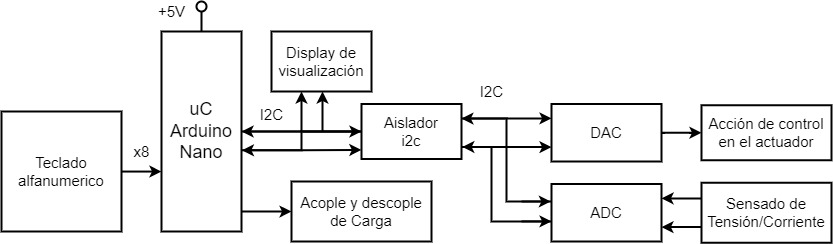
\includegraphics[scale=0.5]{./imagenes/diagrama_digital.jpg}
    \caption{Estructura de archivos de la plantilla.}
    \label{F:diagrama_digital}
\end{figure}

\section{Componentes de la etapa digital.}

\subsection{dsPIC30F4011. High-Performance, 16-Bit Digital Signal Controllers.}
El dsPIC30F4011 es un controlador digital de señales de 16 bits, reconocido por su alto rendimiento y sus amplias capacidades. Diseñado por Microchip Technology, este dispositivo se destaca por su versatilidad, lo que lo convierte en una opción ideal para una variedad de aplicaciones en el ámbito industrial, comercial y de consumo.
Con su arquitectura avanzada y su conjunto completo de características, el dsPIC30F4011 ofrece un rendimiento excepcional en aplicaciones que requieren un control preciso y eficiente de señales digitales. Su capacidad para manejar operaciones complejas en tiempo real lo hace adecuado para una amplia gama de proyectos, desde sistemas de control hasta aplicaciones de procesamiento de señales. Esta también se destaca por su tamaño compacto y su diseño robusto, lo que lo hace fácil de integrar en una variedad de dispositivos y sistemas electrónicos. Además, su amplio rango de temperatura de funcionamiento y su bajo consumo de energía lo hacen adecuado para aplicaciones en entornos exigentes.

\underline{programación}
La programación del dsPIC30F4011 se lleva a cabo utilizando el software MPLAB IDE v8.91, desarrollado por Microchip Technology Incorporated en los Estados Unidos. MPLAB IDE proporciona un entorno de desarrollo integrado (IDE) que facilita la creación, depuración y programación de aplicaciones para microcontroladores de la familia dsPIC.
Este software ofrece una variedad de herramientas y características que simplifican el proceso de desarrollo de software para el dsPIC30F4011, incluyendo un editor de código, compilador, depurador y simulador. Además, MPLAB IDE es compatible con una amplia gama de dispositivos de Microchip, lo que lo convierte en una opción versátil para los desarrolladores de sistemas embebidos.
El código utilizado en el dsPIC30F4011 está disponible en [insertar referencia aquí], que es un enlace a un repositorio en GitHub. Este repositorio contiene el algoritmo desarrollado en los capítulos anteriores, permitiendo a los interesados examinar y comprender el funcionamiento del sistema implementado. La disponibilidad del código fuente en un repositorio público facilita la colaboración, revisión y mejora continua del proyecto, además de proporcionar una referencia para futuros desarrollos y aplicaciones relacionadas con el dsPIC30F4011.

Protocolo de comunicación.
El protocolo de comunicación es fundamental en el diseño y desarrollo de sistemas embebidos, ya que define la manera en que los dispositivos intercambian información entre sí. En el caso del dsPIC30F4011, se cuenta con diversas opciones de protocolos de comunicación, cada uno con sus propias características y aplicaciones específicas.
Entre los protocolos de comunicación compatibles con el dsPIC30F4011 se encuentran:
SPI™ (Serial Peripheral Interface): Permite la comunicación síncrona entre dispositivos mediante una línea de reloj común y líneas separadas para datos de entrada y salida.
I2C™ (Inter-Integrated Circuit): Proporciona una interfaz de comunicación de bus de dos cables que permite la comunicación entre múltiples dispositivos conectados al mismo bus.
Universal Asynchronous Receiver Transmitter (UART): Permite la comunicación serial asíncrona entre el dsPIC30F4011 y otros dispositivos periféricos.
CAN (Controller Area Network): Es un protocolo de comunicación serial diseñado para aplicaciones de control en tiempo real, especialmente en entornos automotrices e industriales.
Para este proyecto en particular, se optará por emplear el protocolo I2C debido a su compatibilidad con los componentes utilizados en la fuente. La elección de este protocolo se fundamenta en su eficiencia y versatilidad, lo que lo hace idóneo para satisfacer los requisitos de comunicación de este sistema embebido.

\begin{figure}[H]
    \centering 
    
\includegraphics[scale=0.5]{./imagenes/mplab.jpg}
    \caption{Logo MPLAB IDE.}
    \label{F:LogoMPLAB}
\end{figure}

\subsection{Teclado de membrana 4x4.}
El teclado de membrana matricial 4x4 autoadhesivo es un dispositivo de entrada que se utiliza comúnmente en aplicaciones electrónicas donde se requiere una interfaz de usuario simple y compacta. Consiste en una delgada lámina de material flexible que contiene una matriz de botones dispuestos en filas y columnas, con un total de 16 botones en este caso particular (4 filas x 4 columnas).
Cada botón en el teclado de membrana está interconectado mediante una disposición de líneas conductoras en la membrana. Estas líneas están organizadas de manera que forman una matriz, permitiendo la detección de la ubicación específica de la tecla presionada. El funcionamiento del teclado de membrana matricial implica un proceso de escaneo continuo de todas las filas y columnas para detectar la presencia de un botón presionado. Cuando un botón se presiona, se cierra un circuito entre la fila y la columna correspondientes, lo que indica al microcontrolador la ubicación de la tecla activada.

\begin{figure}
    \centering [H]
    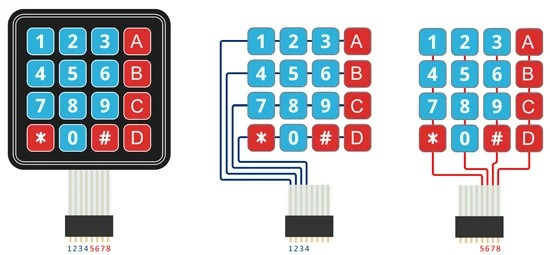
\includegraphics[scale=0.5]{./imagenes/Teclado Matricial 4x4_2.jpg}
    \caption{Estructura de archivos de la plantilla.}
    \label{F:teclado4x4}
\end{figure}

\subsection{Display OLED SSD1306.}
El display OLED SSD1306 elegido para el proyecto utiliza comunicación I2C y ofrece una resolución de 128x64 píxeles. En la Figura 4.13 se presenta una imagen del display, que opera dentro de un rango de voltaje de 3.3 a 5.5 V, lo cual lo hace compatible con el microcontrolador seleccionado. En esta pantalla se mostrará tanto el menú de funcionamiento los modos de operación como un indicador a tiempo real de las magnitudes registradas. Será el vínculo principal entre el usuario y la fuente.

\begin{figure} [H]
    \centering 
    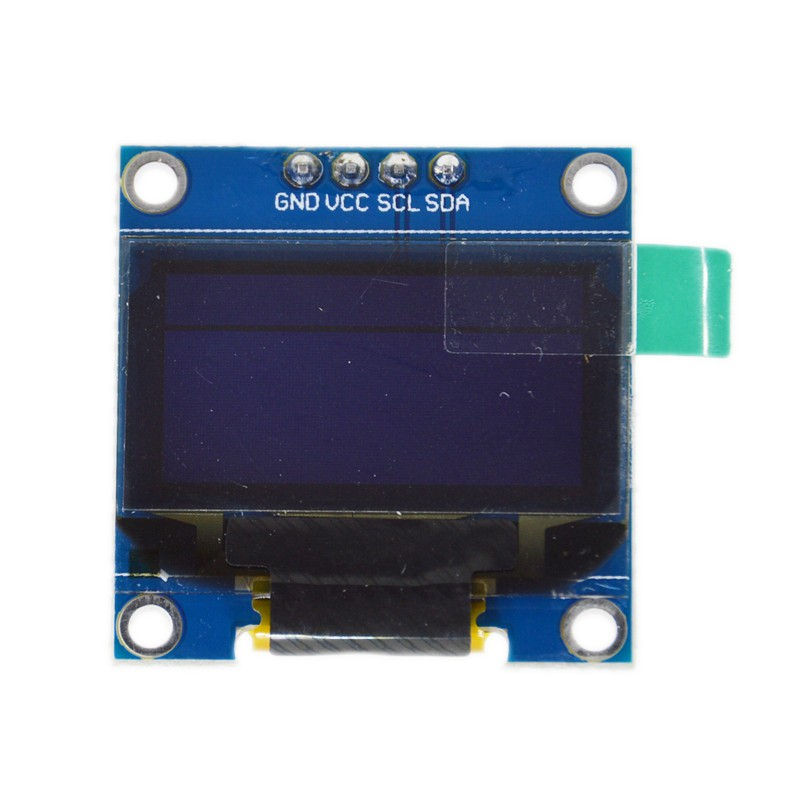
\includegraphics[scale=0.1]{./imagenes/display.jpg}
    \caption{Display OLED SSD1306.}
    \label{F:display}
\end{figure}

\subsection{Aislador I2C capacitivo.}
El dispositivo a utilizar es un ISO1540 [insertar referencia] el cual cuenta con buffers de entrada y salida que están separados por tecnología de aislamiento capacitivo de Texas Instruments que utiliza una barrera de dióxido de silicio (SiO2). Cuando se utilizan con fuentes de alimentación aisladas, estos dispositivos bloquean voltajes altos, aíslan tierras y evitan corrientes de ruido que puedan ingresar a la tierra local e interferir o dañar circuitos sensibles. Esta tecnología de aislamiento ofrece ventajas en función, rendimiento, tamaño y consumo de energía en comparación con los optoacopladores.
De este modo tendremos la aislación galvánica para separar apropiadamente la parte de potencia de la de control.
\begin{figure}[H]
    \centering
    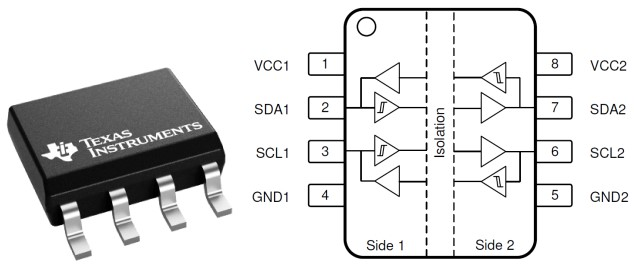
\includegraphics[scale=0.1]{./imagenes/optoi2c.jpg}
    \caption{Aislador capacitivo I2C ISO1540.}
    \label{F:optoi2c}
\end{figure}

\subsection{Convertidor analógico digital. AD.}
El ADS1115 es un componente crucial en la transición de una fuente de alimentación de corriente continua de analógica a digital. Este dispositivo ofrece una impresionante precisión de 16 bits, junto con una velocidad de muestreo de hasta 860 muestras por segundo a través del protocolo de comunicación I2C. Configurable para operar con cuatro canales de entrada de un solo extremo o dos canales diferenciales, el ADS1115 se destaca por su versatilidad en la medición de señales analógicas en entornos digitales. 
Equipado con un conversor delta-sigma de 16 bits, un comparador programable con salida directa al pin de alerta, y una ganancia ajustable que permite la lectura de hasta 256mV en escala completa, este dispositivo garantiza una captura precisa de los datos analógicos. Su interfaz de comunicación I2C facilita la lectura de datos digitales, mientras que su dirección predeterminada de 0x48 y la disponibilidad de bibliotecas para plataformas como Arduino lo convierten en una opción conveniente y de fácil integración en proyectos electrónicos.
\begin{figure}[H]
    \centering
    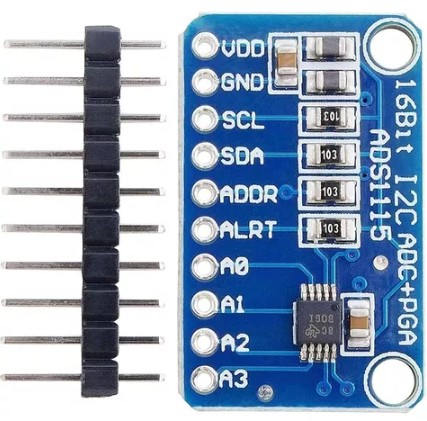
\includegraphics[scale=0.1]{./imagenes/ads1115.jpg}
    \caption{Convertidor AD ADS1115.}
    \label{F:ADC}
\end{figure}

\subsection{Modos de funcionamiento.}
El sistema de control de la fuente de alimentación implementa varios modos de funcionamiento para adaptarse a diversas necesidades de aplicación. A continuación, se describen los principales modos de operación:
Modo Tensión:
En este modo, la fuente de alimentación establece inicialmente el valor máximo de tensión deseado. Posteriormente, limita la corriente máxima de umbral que la carga podrá obtener. Este modo es especialmente útil cuando se requiere controlar la tensión suministrada a la carga de manera precisa y garantizar la seguridad del sistema al limitar la corriente máxima.
Modo Corriente:
En el modo de corriente, la fuente de alimentación establece y controla la corriente suministrada a la carga. Este modo es útil en situaciones donde es crítico mantener la corriente dentro de ciertos límites para proteger los componentes de la carga y garantizar su correcto funcionamiento.
Modo Rampa:
El modo de rampa tiene como objetivo generar un aumento gradual y lineal de la tensión suministrada a la carga durante un período de tiempo determinado. Los parámetros configurables en este modo incluyen la tensión final deseada y el tiempo en el cual se alcanzará esta tensión desde un valor inicial de 0V. Este modo es útil en aplicaciones donde se requiere un inicio suave del sistema para evitar sobrecargas o picos de corriente al arrancar la carga.


\input{contenido/8_software_y_diseño.tex}
\input{contenido/Instrucciones_uso.tex}


%\input{contenido/4_clasificacion_y_def.tex}

% 9. BILIOGRAFÍA
\printbibliography[title={Bibliografía}]

% 8. APÉNDICES
\appendix
% si necesitamos agregar algún apéndice activamos esto
\chapter{Apéndice de ejemplo}
\label{C:anexo-comunicación-serial}

\lipsum[2-4]



\backmatter

%%%%%%%%%%%%%%%%%%%
\end{document}
%%%%%%%%%%%%%%%%%%%
